% ******************************* PhD Thesis Template **************************
% Please have a look at the README.md file for info on how to use the template

\documentclass[a4paper,12pt,times,numbered,print,index, custombib]{Classes/PhDThesisPSnPDF}

% ******************************************************************************
% ******************************* Class Options ********************************
% *********************** See README for more details **************************
% ******************************************************************************

% `a4paper'(The University of Cambridge PhD thesis guidelines recommends a page
% size a4 - default option) or `a5paper': A5 Paper size is also allowed as per
% the Cambridge University Engineering Deparment guidelines for PhD thesis
%
% `11pt' or `12pt'(default): Font Size 10pt is NOT recommended by the University
% guidelines
%
% `oneside' or `twoside'(default): Printing double side (twoside) or single
% side.
%
% `print': Use `print' for print version with appropriate margins and page
% layout. Leaving the options field blank will activate Online version.
%
% `index': For index at the end of the thesis
%
% `draftclassic': For draft mode without loading any images (same as draft in book)
%
% `draft': Special draft mode with line numbers, images, and water mark with
% timestamp and custom text. Position of the text can also be modified.
%
% `abstract': To generate only the title page and abstract page with
% dissertation title and name, to submit to the Student Registry
%
% `chapter`: This option enables only the specified chapter and it's references
%  Useful for review and corrections.
%
% ************************* Custom Page Margins ********************************
%
% `custommargin`: Use `custommargin' in options to activate custom page margins,
% which can be defined in the preamble.tex. Custom margin will override
% print/online margin setup.
%
% *********************** Choosing the Fonts in Class Options ******************
%
% `times' : Times font with math support. (The Cambridge University guidelines
% recommend using times)
%
% `fourier': Utopia Font with Fourier Math font (Font has to be installed)
%            It's a free font.
%
% `customfont': Use `customfont' option in the document class and load the
% package in the preamble.tex
%
% default or leave empty: `Latin Modern' font will be loaded.
%
% ********************** Choosing the Bibliography style ***********************
%
% `authoryear': For author-year citation eg., Krishna (2013)
%
% `numbered': (Default Option) For numbered and sorted citation e.g., [1,5,2]
%
% `custombib': Define your own bibliography style in the `preamble.tex' file.
%              `\RequirePackage[square, sort, numbers, authoryear]{natbib}'.
%              This can be also used to load biblatex instead of natbib
%              (See Preamble)
%
% **************************** Choosing the Page Style *************************
%
% `default (leave empty)': For Page Numbers in Header (Left Even, Right Odd) and
% Chapter Name in Header (Right Even) and Section Name (Left Odd). Blank Footer.
%
% `PageStyleI': Chapter Name next & Page Number on Even Side (Left Even).
% Section Name & Page Number in Header on Odd Side (Right Odd). Footer is empty.
%
% `PageStyleII': Chapter Name on Even Side (Left Even) in Header. Section Number
% and Section Name in Header on Odd Side (Right Odd). Page numbering in footer


% ********************************** Preamble **********************************
% Preamble: Contains packages and user-defined commands and settings
% ******************************************************************************
% ****************************** Custom Margin *********************************

% Add `custommargin' in the document class options to use this section
% Set {innerside margin / outerside margin / topmargin / bottom margin}  and
% other page dimensions
\ifsetCustomMargin
  \RequirePackage[left=35mm,right=20mm,top=25mm,bottom=25mm]{geometry}
  \setFancyHdr % To apply fancy header after geometry package is loaded
\fi

% Add spaces between paragraphs
%\setlength{\parskip}{0.5em}
% Ragged bottom avoids extra whitespaces between paragraphs
\raggedbottom
% To remove the excess top spacing for enumeration, list and description
%\usepackage{enumitem}
%\setlist[enumerate,itemize,description]{topsep=0em}

% *****************************************************************************
% ******************* Fonts (like different typewriter fonts etc.)*************

% Add `customfont' in the document class option to use this section

%\ifsetCustomFont
  % Set your custom font here and use `customfont' in options. Leave empty to
  % load computer modern font (default LaTeX font).
  %
%  \RequirePackage{helvet}

  % For use with XeLaTeX
  %  \setmainfont[
  %    Path              = ./libertine/opentype/,
  %    Extension         = .otf,
  %    UprightFont = LinLibertine_R,
  %    BoldFont = LinLibertine_RZ, % Linux Libertine O Regular Semibold
  %    ItalicFont = LinLibertine_RI,
  %    BoldItalicFont = LinLibertine_RZI, % Linux Libertine O Regular Semibold Italic
  %  ]
  %  {libertine}
  %  % load font from system font
  %  \newfontfamily\libertinesystemfont{Linux Libertine O}
%\fi

% *****************************************************************************
% **************************** Custom Packages ********************************

% ************************* Algorithms and Pseudocode **************************
%\usepackage{xltxtra}
%\usepackage{algpseudocode}


% ********************Captions and Hyperreferencing / URL **********************

% Captions: This makes captions of figures use a boldfaced small font.
%\RequirePackage[small,bf]{caption}

\RequirePackage[labelsep=space,tableposition=top]{caption}
\renewcommand{\figurename}{Fig.} %to support older versions of captions.sty


% *************************** Graphics and figures *****************************
\usepackage{float}
%\usepackage{rotating}
%\usepackage{wrapfig}

% Uncomment the following two lines to force Latex to place the figure.
% Use [H] when including graphics. Note 'H' instead of 'h'
%\usepackage{float}
%\restylefloat{figure}
\usepackage[labelfont=bf]{caption}
% Subcaption package is also available in the sty folder you can use that by
% uncommenting the following line
% This is for people stuck with older versions of texlive
%\usepackage{sty/caption/subcaption}
\usepackage{subcaption}
\usepackage{listings}
\lstdefinestyle{sharpc}{language=[Sharp]C, frame=lr, rulecolor=\color{blue!80!black}}

% ********************************** Tables ************************************
\usepackage{booktabs} % For professional looking tables
\usepackage{multirow}
\usepackage[table]{xcolor}

%\usepackage{multicol}
%\usepackage{longtable}
%\usepackage{tabularx}


% *********************************** SI Units *********************************
\usepackage{siunitx} % use this package module for SI units


% ******************************* Line Spacing *********************************

% Choose linespacing as appropriate. Default is one-half line spacing as per the
% University guidelines

% \doublespacing
% \onehalfspacing
 \singlespacing


% ************************ Formatting / Footnote *******************************

% Don't break enumeration (etc.) across pages in an ugly manner (default 10000)
%\clubpenalty=500
%\widowpenalty=500

%\usepackage[perpage]{footmisc} %Range of footnote options


% *****************************************************************************
% *************************** Bibliography  and References ********************

%\usepackage{cleveref} %Referencing without need to explicitly state fig /table

% Add `custombib' in the document class option to use this section
\ifuseCustomBib
   \RequirePackage[square, sort, numbers, authoryear]{natbib} % CustomBib

% If you would like to use biblatex for your reference management, as opposed to the default `natbibpackage` pass the option `custombib` in the document class. Comment out the previous line to make sure you don't load the natbib package. Uncomment the following lines and specify the location of references.bib file

%\RequirePackage[backend=biber, style=numeric-comp, citestyle=numeric, sorting=nty, natbib=true]{biblatex}
%\bibliography{References/references} %Location of references.bib only for biblatex

\fi
\usepackage{url}
% changes the default name `Bibliography` -> `References'
\renewcommand{\bibname}{References}


% ******************************** Roman Pages *********************************
% The romanpages environment set the page numbering to lowercase roman one
% for the contents and figures lists. It also resets
% page-numbering for the remainder of the dissertation (arabic, starting at 1).

\newenvironment{romanpages}{
  \setcounter{page}{1}
  \renewcommand{\thepage}{\roman{page}}}
{\newpage\renewcommand{\thepage}{\arabic{page}}}


% ******************************************************************************
% ************************* User Defined Commands ******************************
% ******************************************************************************
\usepackage{epigraph}
\usepackage{tikz}
\usepackage{pgf-pie}

% *********** To change the name of Table of Contents / LOF and LOT ************

\renewcommand{\contentsname}{List of Contents}
%\renewcommand{\listfigurename}{My List of Figures}
%\renewcommand{\listtablename}{My List of Tables}

% *****************************************************************************
% *************** Changing the Visual Style of Chapter Headings ***************

% This section on visual style is from https://github.com/cambridge/thesis

% Uncomment the section below. Requires titlesec package.

%\RequirePackage{titlesec}


\usepackage[T1]{fontenc}
\usepackage{sectsty}
\chapterfont{\fontfamily{mdpgd}\selectfont} %% for chapter if you want
\sectionfont{\fontfamily{mdpgd}\selectfont}
\subsectionfont{\fontfamily{mdpgd}\selectfont} %% Similarly for others. see the manual of sectsty, section 5.


%\usepackage{titlesec}
%\titleformat{\chapter}[display]
%  {\fontfamily{garamondx}}
%  {\chaptertitlename\ \thechapter}
%  {20pt}
%  {}
%\titleformat{\section}
%  {\fontfamily{garamondx}\selectfont\bfseries\Large}
%  {\thesection}
%  {1em}
%  {}
%\titleformat{\subsection}
%  {\fontfamily{garamondx}\selectfont\bfseries\Large}
%  {\thesection}
%  {1em}
%  {}
%\newcommand{\PreContentTitleFormat}{\titleformat{\chapter}[display]{\scshape\Large}
%{\Large\filleft{\chaptertitlename} \Huge\thechapter}
%{1ex}{}
%[\vspace{1ex}\titlerule]}
%\newcommand{\ContentTitleFormat}{\titleformat{\chapter}[display]{\scshape\huge}
%{\Large\filleft{\chaptertitlename} \Huge\thechapter}{1ex}
%{\titlerule\vspace{1ex}\filright}
%[\vspace{1ex}\titlerule]}
%\newcommand{\PostContentTitleFormat}{\PreContentTitleFormat}
%\PreContentTitleFormat


% ********************** TOC depth and numbering depth *************************

\setcounter{secnumdepth}{2}
\setcounter{tocdepth}{2}


% ******************************* Nomenclature *********************************

% To change the name of the Nomenclature section, uncomment the following line
\usepackage{nomencl}
\makenomenclature
%\renewcommand{\nomlabel}[1]{\texttt{#1}}

%\renewcommand{\nomname}{List of abbreviations}


% ********************************* Appendix ***********************************

% The default value of both \appendixtocname and \appendixpagename is `Appendices'. These names can all be changed via:

%\renewcommand{\appendixtocname}{List of appendices}
%\renewcommand{\appendixname}{Appndx}

% *********************** Configure Draft Mode **********************************

% Uncomment to disable figures in `draftmode'
%\setkeys{Gin}{draft=true}  % set draft to false to enable figures in `draft'

% These options are active only during the draft mode
% Default text is "Draft"
%\SetDraftText{DRAFT}

% Default Watermark location is top. Location (top/bottom)
%\SetDraftWMPosition{bottom}

% Draft Version - default is v1.0
%\SetDraftVersion{v1.1}

% Draft Text grayscale value (should be between 0-black and 1-white)
% Default value is 0.75
%\SetDraftGrayScale{0.8}


% ******************************** Todo Notes **********************************
%% Uncomment the following lines to have todonotes.

%\ifsetDraft
%	\usepackage[colorinlistoftodos]{todonotes}
%	\newcommand{\mynote}[1]{\todo[author=kks32,size=\small,inline,color=green!40]{#1}}
%\else
%	\newcommand{\mynote}[1]{}
%	\newcommand{\listoftodos}{}
%\fi

% Example todo: \mynote{Hey! I have a note}


% ************************ Thesis Information & Meta-data **********************
% Thesis title and author information, refernce file for biblatex
%% ************************ Thesis Information & Meta-data **********************
%% The title of the thesis
\title{Writing your PhD thesis in \texorpdfstring{\\ \LaTeX2e}{LaTeX2e}}
%\texorpdfstring is used for PDF metadata. Usage:
%\texorpdfstring{LaTeX_Version}{PDF Version (non-latex)} eg.,
%\texorpdfstring{$sigma$}{sigma}

%% Subtitle (Optional)
\subtitle{Using the CUED template}

%% The full name of the author
\author{Krishna Kumar}

%% Department (eg. Department of Engineering, Maths, Physics)
\dept{Department of Engineering}

%% University and Crest
\university{University of Cambridge}
% Crest minimum should be 30mm.
\crest{
\includegraphics[width=0.2\textwidth]{University_Crest}}
%% Use this crest, if you are using the college crest
%% Crest long miminum should be 65mm
%\crest{
\includegraphics[width=0.45\textwidth]{University_Crest_Long}}

%% College shield [optional] 
% Crest minimum should be 30mm.
%\collegeshield{
\includegraphics[width=0.2\textwidth]{CollegeShields/Kings}}


%% Supervisor (optional)
%\supervisor{Prof. Kenichi Soga}
%% Supervisor Role (optional) - Supervisor (default) or advisor
%\supervisorrole{Advisor: }

%% Advisor (optional)
%\advisor{Prof. Malcolm Bolton}
%% Advisor Role (optional) - Advisor (default) or leave empty
%\advisorrole{Advisor: }


%% You can redefine the submission text:
% Default as per the University guidelines:
% ``This dissertation is submitted for the degree of''
%\renewcommand{\submissiontext}{change the default text here if needed}

%% Full title of the Degree
\degreetitle{Doctor of Philosophy}

%% College affiliation (optional)
\college{King's College}

%% Submission date
% Default is set as {\monthname[\the\month]\space\the\year}
%\degreedate{September 2014} 

%% Meta information
\subject{LaTeX} \keywords{{LaTeX} {PhD Thesis} {Engineering} {University of
Cambridge}}


% ***************************** Abstract Separate ******************************
% To printout only the titlepage and the abstract with the PhD title and the
% author name for submission to the Student Registry, use the `abstract' option in
% the document class.

%\ifdefineAbstract
% \pagestyle{empty}
% \includeonly{Declaration/declaration, Abstract/abstract}
%\fi

% ***************************** Chapter Mode ***********************************
% The chapter mode allows user to only print particular chapters with references
% Title, Contents, Frontmatter are disabled by default
% Useful option to review a particular chapter or to send it to supervisior.
% To use choose `chapter' option in the document class

\ifdefineChapter
 \includeonly{Chapter3/chapter3}
\fi
% ***************************** Removing epigraph style from a page ***********************************
\makeatletter
\renewcommand{\epigraphhead}[2][95]{%
  \def\@epitemp{\begin{minipage}{\epigraphwidth}#2\end{minipage}}
  \def\ps@epigraph{\let\@mkboth\@gobbletwo
    \@epipos
    \if@epirhs
      \def\@oddhead{\hfil\begin{picture}(0,0)
                         \put(0,-#1){\makebox(0,0)[r]{\@epitemp}}
                         \end{picture}}
    \else
      \if@epicenter
        \def\@oddhead{\hfil\begin{picture}(0,0)
                           \put(0,-#1){\makebox(0,0)[b]{\@epitemp}}
                           \end{picture}\hfil}
      \else
        \def\@oddhead{\begin{picture}(0,0)
                           \put(0,-#1){\makebox(0,0)[l]{\@epitemp}}
                           \end{picture}\hfil}
      \fi
    \fi
    \let\@evenhead\@oddhead
    \def\@oddfoot{\reset@font}
    \let\@evenfoot\@oddfoot}
  \thispagestyle{epigraph}}
\makeatother


% ******************************** Front Matter ********************************
\begin{document}

\frontmatter

%\begin{titlepage}
%  \maketitle
%\end{titlepage}


%% ******************************* Thesis Dedidcation ********************************

\begin{dedication} 

I would like to dedicate this thesis to my loving parents \dots

\end{dedication}


%% ******************************* Thesis Declaration ***************************

\begin{declaration}

I hereby declare that except where specific reference is made to the work of 
others, the contents of this dissertation are original and have not been 
submitted in whole or in part for consideration for any other degree or 
qualification in this, or any other university. This dissertation is my own 
work and contains nothing which is the outcome of work done in collaboration 
with others, except as specified in the text and Acknowledgements. This 
dissertation contains fewer than 65,000 words including appendices, 
bibliography, footnotes, tables and equations and has fewer than 150 figures.

% Author and date will be inserted automatically from thesis.tex \author \degreedate

\end{declaration}


%% ************************** Thesis Acknowledgements **************************

\begin{acknowledgements}      


And I would like to acknowledge ...


\end{acknowledgements}

%% ************************** Thesis Abstract *****************************
% Use `abstract' as an option in the document class to print only the titlepage and the abstract.
\begin{abstract}
This is where you write your abstract ...
\end{abstract}


% *********************** Adding TOC and List of Figures ***********************

\tableofcontents

%\listoffigures

%\listoftables

% \printnomenclature[space] space can be set as 2em between symbol and description
\printnomenclature[6em]
%\printnomenclature


% ******************************** Main Matter *********************************
\mainmatter
%\printnomenclature
\makenomenclature
%\textbf{AR} - Augmented Reality\\
%\textbf{AV} - Augmented Virtuality\\
%\textbf{CPU} - Central Processing Unit\\
%\textbf{DOF} - Degree of Freedom\\
%\textbf{EOG} - Electro-Oculography\\
%\textbf{FOV} - Field of View\\
%\textbf{GPU} - Graphics Processing Unit\\
%\textbf{HMD} - Head-Mounted Display\\
%\textbf{IDE} - Integrated Development Environment\\
%\textbf{IR} - Infrared\\
%\textbf{LOD} - Level of Detail\\
%\textbf{MR} - Mixed Reality\\
%\textbf{RE} - Real Environment\\
%\textbf{SDK} - Software Development Kit\\
%\textbf{VE} - Virtual Environment\\
%\textbf{VR} - Virtual Reality\\
%\textbf{WOW} - Window on World\\
%*******************************************************************************
%*********************************** First Chapter *****************************
%*******************************************************************************

\chapter{Virtual reality – theoretical background}\label{chapter1}  %Title of the First Chapter

\epigraphhead[40]{\epigraph{\textit{Reality is merely an illusion, albeit \linebreak a very persistent one.}}{{Albert Einstein}}}

\ifpdf
    \graphicspath{{Chapter1/Figs/Raster/}{Chapter1/Figs/PDF/}{Chapter1/Figs/}}
\else
    \graphicspath{{Chapter1/Figs/Vector/}{Chapter1/Figs/}}
\fi


%********************************** %First Section  **************************************
\section{Definition} %Section - 1.1 

	Nowadays, thanks to constant technology development, accessibility of Internet and computer-related innovations, people
tend to live parallelly in two worlds- real and virtual. As the latter one offers less boundaries and constraints, and the only limit there is, is people's imagination, it is not surprising that these days one can observe growing trend in improving the quality of man's immersion in artificial world. This possibility leads to the new idea of perceiving the surrounding reality, which is called Virtual Reality (VR) or Virtual Environment (VE).

	The concept of VR has never been unified, therefore it cannot be defined in one way. One of the most general definition explains it as "an immersive and interactive system that provides users with the illusion of entering a virtual world" \cite{Heim98}. In other papers one can find more specific description. Most of them state that three- dimensional graphics is an essential part of VR \cite{Fuchs92}, moreover, that it needs to provide a multi-sensory computer-mediated environment \cite{Cruz93}. Despite the multitude of possible definitions, all of them agree that VE is immersive, interactive and that it creates an experience in simulated world. It is well systematized by Sherman and Craig \cite{Sherman03}, who describe four essential elements in VR, which are:
\begin{itemize}
\item \textbf{Virtual world}– set of objects in a space, relationship between them and laws that govern this entirety.
\item \textbf{Immersion}– impression of being present in showed environment instead of looking at it from the outside. This phenomenon will be described more precisely in section \ref{imm}.
\item \textbf{Sensory feedback}– collection of sensory data about the environment based on user input, for example his position which determines the given view and perspective.
\item \textbf{Interactivity}– responsiveness to user actions.
\end{itemize}
Those features of Virtual Reality draw it away from traditional media technologies and thus VE gives new possibilities which has never been considered before.
	
	In this section it is worth mentioning other notions, closely related to VR, which are Real Enovironment (RE), Mixed Reality (MR) Augmented Reality (AR) and Augmented Virtuality (AV). For this purpose it is convenient to introduce the concept of Reality-Virtuality Continuum, which is presented below, in Figure \ref{fig:continuum}.
\begin{figure}[h] 
\centering    
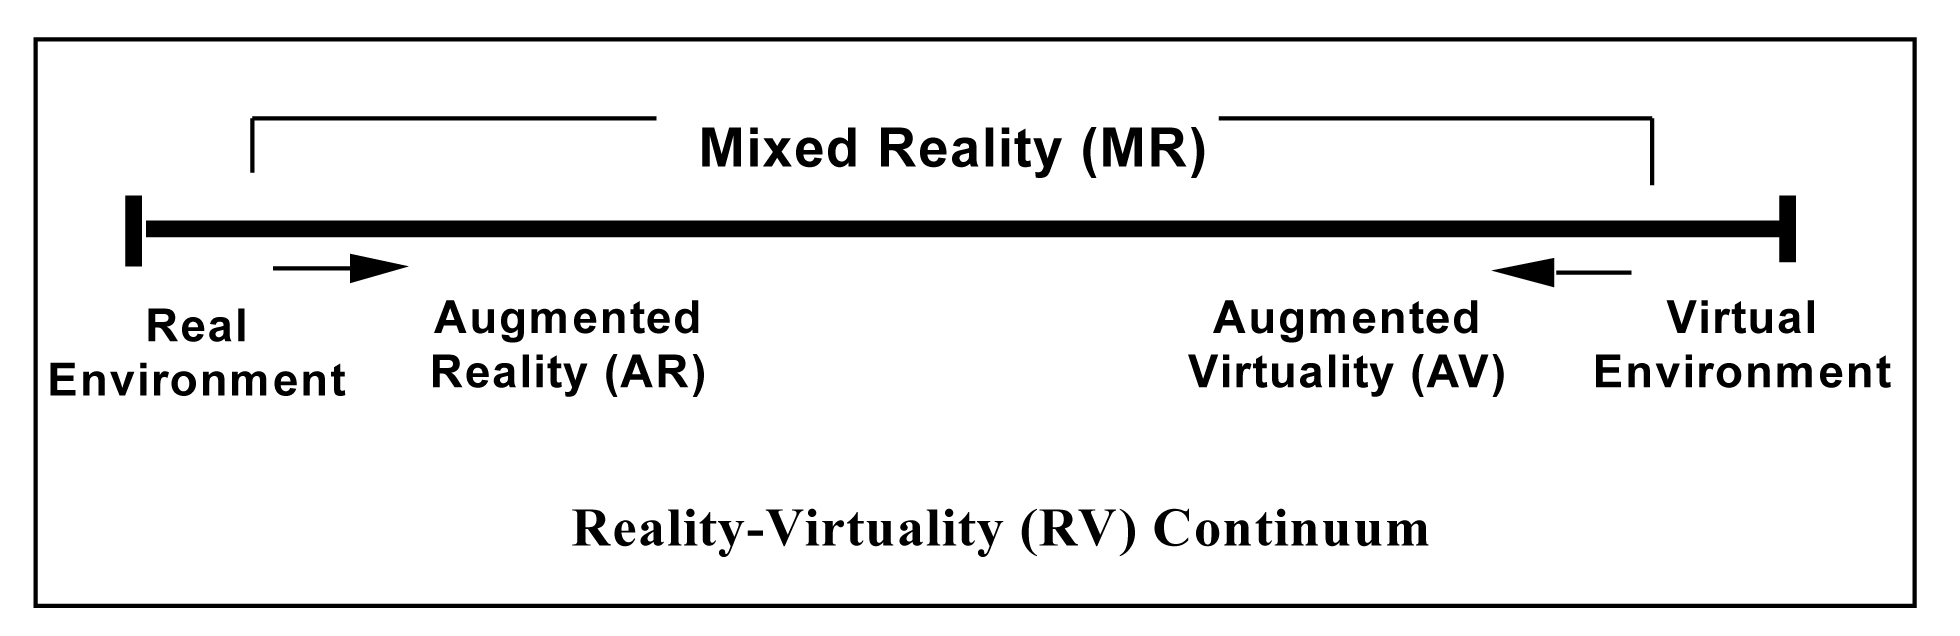
\includegraphics[width=1.0\textwidth]{Figs/rv_continuum.jpg}
\caption{Representation of Reality-Virtuality Continuum \cite{Milgram94}.}
\label{fig:continuum}
\end{figure}
\\As shown, the Real Environment is an opposite idea to the one that was already explained, which is Virtual Reality. Thus one can understand it as an environment, which consists of the real objects exclusively, observed either in person or through some kind of display or window. Between those two extrema of RV, the Mixed Reality is placed. It is a general notion, which describes surrounding, where both real and virtual objects are presented together. While going into details, two subconcepts occur. First one, Augmented Reality, may be defined as "augmenting natural feedback to the operator with simulated cues" \cite{Milgram94}, what practically means that the user display is transparent, so it shows the view of a real world, but additionally enriched with coexisting virtual objects. Ipso facto, Augmented Virtuality is very close to AR, as the only difference between them is stated by proportions of virtuality and reality presented to the user, what results from Figure \ref{fig:continuum}. It follows, therefore, that those two concepts interpenetrate.


	 
%********************************** %Second Section  *************************************
\section{History}\label{history} %Section - 1.2 

It may seem that Virtual Reality is an idea that originated with a recent rapid technological development. In fact, VR's origins date back to 1950s at the latest, when the first devices for that purpose were designed.

In 1957 the machine called \textit{Sensorama} (Figure \ref{fig:sensorama})  was constructed by Morton Heiling. This multi-sensory stimulator contained prerecorded film in color and stereo (six to choose), binaural sound and, additionally, scent, wind and vibration effects. Although it was not interactive, \textit{Sensorama} is considered as the first Virtual Environment system.
\begin{figure}[h] 
\centering    
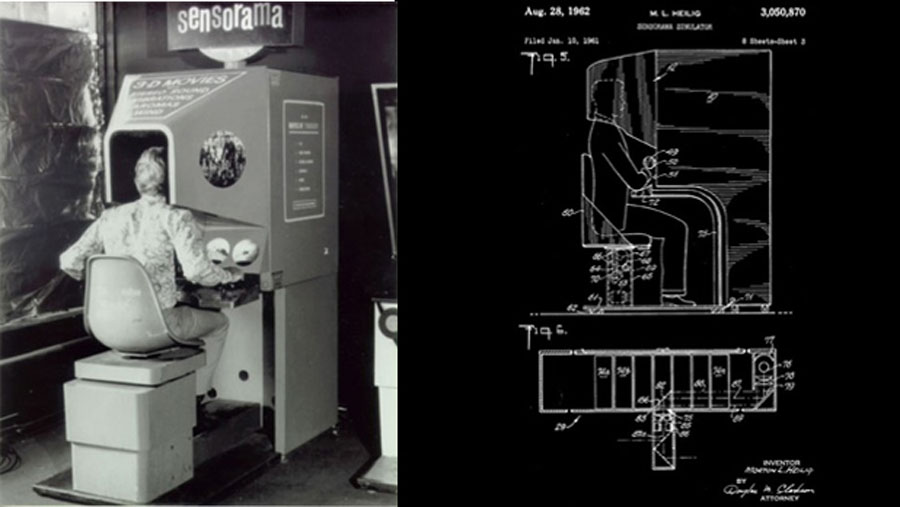
\includegraphics[width=0.8\textwidth]{Figs/sensorama.jpg}
\caption{\textit{Sensorama}, patented in 1962 \cite{Olszewski15}.}
\label{fig:sensorama}
\end{figure}
Four years later, Philico Corporation produced another device- the \textit{Headsight}, which was the first example of Head-Mounted Display (HMD) with motion tracking. It provided a vision of a film that was recorded in a real time by cameras, what makes it an Agumented Reality rather than VR system.
Subsequently, in 1965, Ivan Sutherland, proposed the concept of \textit{The Ultimate Display}. The assumptions he declared, encompass the Virtual Reality idea until today. These were virtual world maintained in real time through a computer hardware, user's ability to interact with it and a tactile feedback, all with usage of HMD and augmented 3D sound. On this basis he created      
\textit{The Sword of Damocles}, device with Head-Mounted Display and head-tracking. Although its large size and weight, it was invested in by NASA and CIA \cite{Olszewski15, Mandal13}.

1970s brought another new, innovative ideas, like \textit{GROPE}- prototype of a force-feedback system or \textit{VIDEOPLACE}- artificial reality, where position-tracked silhouette of a user was projected on a screen as an avatar. But the most rapid development occured in the next decades, when the miniaturisation went hand in hand with expenses reduction. In 1985 and 1988, the VPL company introduced first commercially available VE devices- \textit{DataGlove} and \textit{EyePhone} HMD. Next, in 1989, Fake Space Labs manufactured \textit{BOOM}, which was a small box with two CRT monitors creating the stereoscopic view and a mechanical arm measuring the position of a box, what allows the user move through a virtual world. Another concept, that did not base on Head-Mounted Display, was presented three years later as the \textit{CAVE}- Cave Automatic Virtual Environment. Here, the stereoscopic images were projected on the walls of a room and could be interpreted properly thanks to LCD shutter glasses worn by a user. Comparing to HMD solutions, \textit{CAVE} assured wider field of view and better quality of presented images. In the decade of 1990s the strongest interest was shown in games industry as a VR's application. This resulted into several systems, like \textit{Virtuality}, \textit{Sega VR} or \textit{Virtual Boy}, which often showed poor image quality or even caused adverse health effects (nausea or headache) to the user \cite{Olszewski15, Mandal13}. 

After the strong 3D graphics development, in 2012, young constructor Palmer Luckey created a new HMD-based device called \textit{Oculus Rift}, that met with a great commercial interest. Two years later, Oculus VR company was bought for a 2,5 billion of dollars, what accelerated a present growth of Virtual Reality development \cite{Olszewski15}. Current used software and hardware are described in section \ref{har} and \ref{dev}.
 
%********************************** %Third Section  *************************************
\section{Hardware and software}\label{har}%Section - 1.3

First of all, to understand how does the Virtual Reality really works, one has to become familiar with the basic components of those systems and their architecture. Generally, in VE systems, user is connected as part of the input/output loop, providing input through devices for interaction and experiencing the result of this input through variety of output, immersive devices. VR engine (computer) is responsible for processing loop information in real-time. Figure \ref{fig:architecture} presents the scheme of those dependencies.
\begin{figure}[h]
\centering    
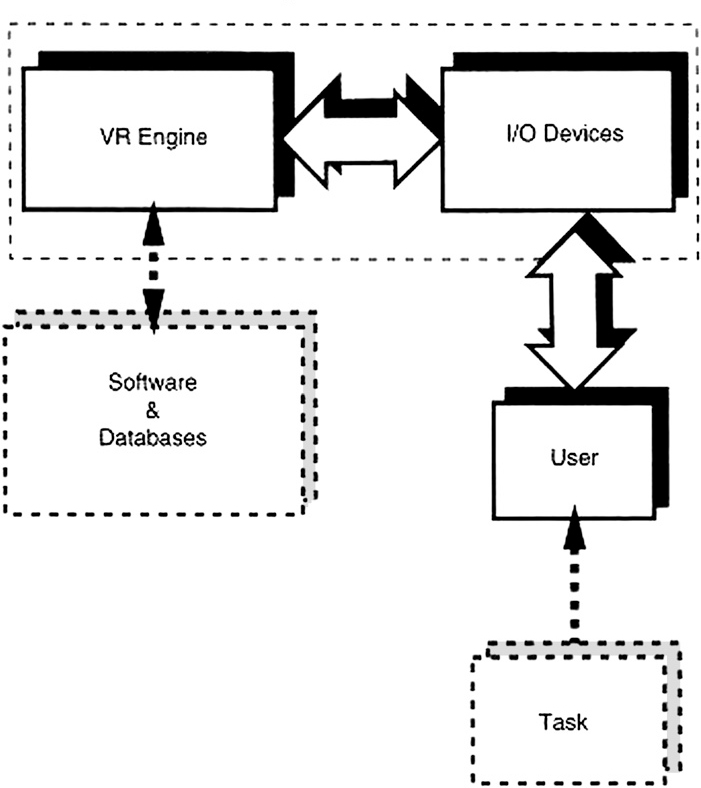
\includegraphics[width=0.5\textwidth]{Figs/architecture.jpg}
\caption{Architecture of Virtual Reality system. I/O stands for input/output \cite{Lange10}.}
\label{fig:architecture} 
\end{figure}
\subsection{Immersion}\label{imm}%Subsection - 1.3.1
Sensation of immersion can differ qualitatively, therefore, on this basis, Virtual Reality is divided into three groups \cite{Mandal13}:

\begin{enumerate}
\item Non-immersive systems
\item Semi-immersive systems
\item Immersive systems
\end{enumerate}

The first one which is called, interchangeably, Desktop-VR systems or WOW (Window on World), is a simplest type of VE. It does not employ special devices, since it is based on working of one or more computer screens (mostly monoscopic). It allows interaction of user, but does not give him an impression of immersion and barely blocks out the real world. Therefore in some quarters it is not considered as Virtual Reality technology. Semi-immersive systems (Fish Tank VR) are improved versions of Desktop-VR, as they use not only screens, which are often stereoscopic in this case, but also head-tracking devices, that intensify immersion of a user. As they do not provide sensory feedback, they cannot be recognized as the third category of systems. Fully immersive systems, besides supporting stereoscopic vision, employ Head-Mounted Display which enables to, according to user input (position, orientation), change the view of the scene. Thanks to that, user may look and move around, so simply navigate in the virtual world which, additionally, is presented in full scale. Moreover, the immersion effect may be upgraded by sensory, auditory and haptic interfaces \cite{Mandal13, Brooks99}. 

Depending on the application and developer invention, user may achieve different types of immersion, which are listed below \cite{Mandal13}:
\begin{itemize}
\item Sensory immersion- feeling of entering into the virtual world and being stimulated intellectually by it. Experience of time and space unity because of the fusion with image medium.
\item Spatial immersion- occurs when the simulated world is perceptually convincing.
\item Narrative immersion- experience of being gripped in a story presented in virtual world.
\item Tactical immersion- occurs when user performs tactile actions that involve skill.
\item Strategic immersion- analytical involvement associated with mental challenge.
\item Psychological immersion- confusing the virtual surrounding with real life.
\end{itemize}
\subsection{Sensory feedback- output}%Subsection - 1.3.2
In simulating artificial world, the most important role plays stimulating user's senses. Thus, knowing the contribution of each one for information passed to humans brain, is very useful. Figure \ref{fig:senses} explains why the visual part of VR has become a focus of research and why the sense of sight appeals to people imagination the most. 
\begin{figure}[h]
\centering
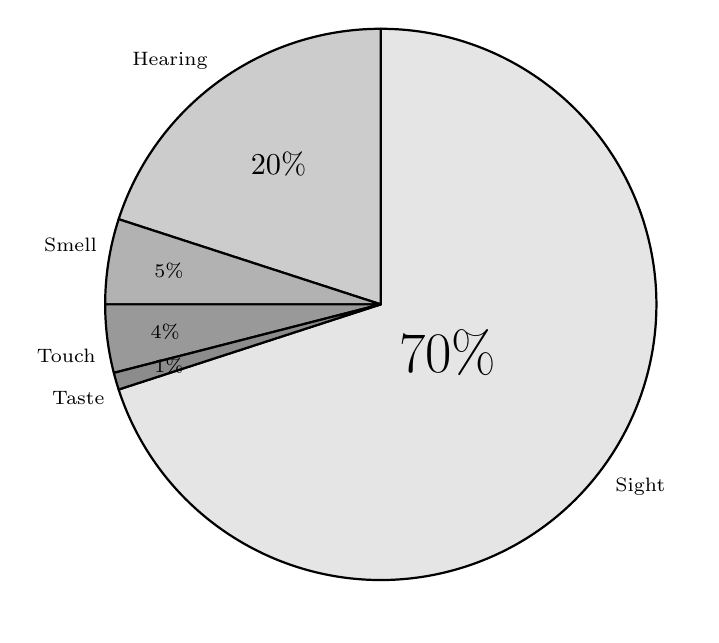
\begin{tikzpicture}
\tikzstyle{every node}=[font=\scriptsize]
\pie [scale font, radius=3.5, rotate = 198, color ={black!10,black!20,black!30,black!40,black!45}] {70/Sight, 20/Hearing, 5/Smell, 4/Touch, 1/Taste}
\end{tikzpicture}
\caption{Five human senses contribution in information transfering to a brain \cite{Mazuryk96}.}
\label{fig:senses}
\end{figure}
Despite this fact, other senses are also taken into consideration of Virtual Environment systems research, what is presented below in this section. 
\subsubsection{Sight}\label{sight}
Human vision is stereoscopic, as each eye can see one two-dimensional image which partly overlap. Those images are being processed by a human brain obtaining a parallax effect- visual phenomenon of depth perception, based on a difference in position of each eye. This phenomena is mimicked by devices simulating three-dimensional vision, the most important ingredient in Virtual Reality- they generate different images for each eye performing natural dimensions and high resolution. 

The simplest gear to obtain stereoscopic vision are anaglyphic glasses. Each lens there has a different color, which acts as color filter, dividing an image in two sub-images. Another device is called shutter glasses, which have LCD screen in front of each eye. They are switched on interchangeably, corresponding with an image presented on a screen resulting in a 3D image \cite{Lacrama07}.
Next example, Fish Tank VR systems, use 3D glasses and standard desktop monitor. In this case, stereoscopic images are created with usage of the off-axis projection, the method that generates two asymmetrical (not centered on the main projection axis) projections.
\begin{figure}[h]
\centering    
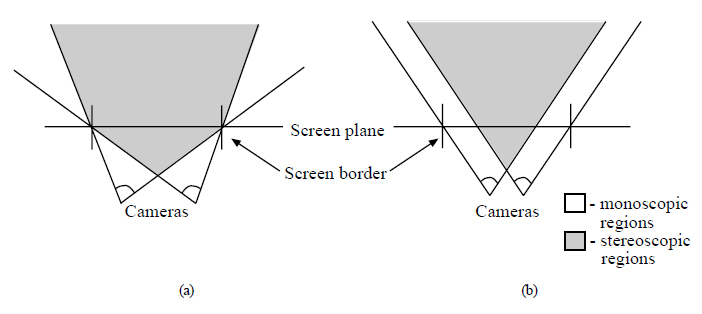
\includegraphics[width=0.9\textwidth]{Figs/projections.jpg}
\caption{Two centers of projection trasnformations: a) off-axis projection b) on-axis projection \cite{Mazuryk96}.}
\label{fig:projections} 
\end{figure} 
Nevertheless, in the subject of Virtual Reality, the most often used devices nowadays are immersive systems, like Head-Mounted Display, where different image displayed for each eye result in a stereoscopic effect. It may be obtained both by on-axis projection (when both image positions are on the symmetry axis of the view plane) or off-axis projection. The latter one is often needed since the tracked head position is not defined only by the axis of view plane. In modern systems the choice is up to the application developer \cite{Mazuryk96, Wikibook15}. The difference between those two approaches is shown in Figure \ref{fig:projections}.

Another issue discussing the vision is the field of view (FOV). Theoretically, human eye retains FOV of 180° both horizontal and vertical. Practically, this value is reduced to 150° because of the obscurement with cheeks, eyebrows and nose. Total horizontal viewing range binocularly overlaps in 120° (when focused on infinity). Since the task of Virtual Reality is to give sensations that are close to real ones, FOV is a parameter of high importance and it may be noticed in HMDs development. As example, current devices use the barrel distortion (Figure \ref{fig:tuscany})- technique that distorts image and enables lenses to present wider FOV, mimicking spherical shape of the eye \cite{Parisi15}.  Typical headset in 1996 supported 40°-60° field of view, while \textit{Oculus Rift} or \textit{HTC Vive} in 2015 covered 110°. For comparison with traditional visualisations, a 21" monitor observed from distance of 50 cm reaches 48° \cite{Mazuryk96, Oscillada15}.
\begin{figure}[h]
\centering    
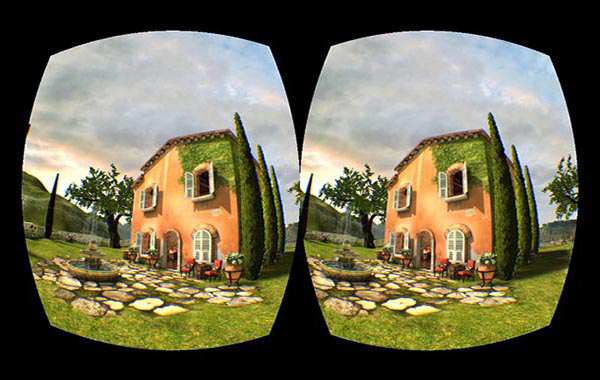
\includegraphics[width=1.0\textwidth]{Figs/tuscany.jpg}
\caption{VR Demo rednered in stereo with \textit{Oculus Rift} using barrel distortion \cite{Parisi15}.}
\label{fig:tuscany} 
\end{figure} 

\subsubsection{Hearing}
When vision does not provide enough information, auditory channel grows in importance. It may give an extra information (enabling perception of data outside the FOV) and may help in spatial orientation. Indeed, 3D sound in VR increases the level of immersion by simulating distances, directions and material information about the surrounding.

Spatial hearing in humans occurs by appraising both monaural (the same for both ears) and binaural (different for each eardrum) clues. The latter occur, if the sound source is placed outside the median plane- the distance between it and each ear is different, causing interaural differences of time (ITD) or intensity (IID). Those phenomenons are mainly used for directivity perception, which is an accurate tool (up to one degree), but only works in case of laterally localizing. On the other hand, monaural cues provide information about elevation: amplifications and attenuations in the frequency bands (intervals in frequency domain). These clues are needed in front/back localization. To recognize the direction in this case, humans rely on spectral modifications of sound caused by the shape and size of a head, neck, torso and outer ears. It is possible since the sound interacts with the body geometry differently, depending on its direction. All these subtle signals received by humans brain through the ears generate the effect of spatial sound perception \cite{Mazuryk96, Gobbetti99, Oculus16}. 

Thus to create a good immersion audio effect, one has to take into account not only the dependencies presented above, as they reffer to directional recognition only. Introducing sound changes while moving past listener (doppler shifts), considering environment geometry, distances (usually as a consequence of loudness) and material properties of objects (which may generate echoes) should also be done. Finally, sound and visual events need to be synchronized \cite{Mazuryk96, Gobbetti99}.
Therefore, to achieve successful acoustic simulation, three basic steps are required \cite{Mazuryk96}:
\begin{enumerate}
\item Sound generation- creating sounds, either by sampling or synthesizing, needed in the virtual world.
\item Spatial propagation- calculation of movement of sound waves through the environment.
\item Mapping of parameters- mapping calculated parameters from second step onto sounds that will be delivered through headphones or speakers to the user, with consideration of monaural and binaural clues to achieve the directional effect.
\end{enumerate}

According to the \textit{Oculus Rift} documentation, to accomplish second and third step in \textit{Oculus} device, the Head-Related Transfer Functions (HRTF) referring to directional recognition are applied. HRTF data may be obtained both experimentally (from human tests) and by head model simulation. Since they are not perfect and often need interpolation of data, mimicking the real spacial sound system is still in a field of study \cite{Oculus16}.
 \subsubsection{Smell}
Although olfactory simulation is not commonly used in Virtual Reality, it may play an important role in some applications of VE, like surgical simulations or simulations designed for emergency medical personnel operating in the field. Human can detect smells in concentration from one part per million up to one part per billion. Additionally, it is much easier to recognize increases than decreases in concentration, therefore VR hardware with olfactory output should enable diffusing odours when needed and, when it is not longer required, purify and filter the air.

The method that makes delivering odours possible is simply odourant storage. They can be stored as liquids, gels or waxes and usually are microencapsulated or compressed on flat surfaces. Metering of the exact amount smell is done by capsules scratching. The whole system should be miniaturised and have low power requirements, as the most convenient would be placing it in HMD \cite{Gobbetti99}. 

Modern olfactory devices for VR are still in the testing phase. One of them, called \textit{The FeelReal}, is supposed to work as an add-on to different kinds of HMD available on the market. It does not only support seven smells (which may be chosen while buying the whole system), but also its temperature, generating hot (e.g. mimicking fire) or cool (e.g. mimicking cool water) scented air \cite{Feelreal16}. 
 \subsubsection{Touch}\label{touch}
The last sense discussed in this section is touch, as it may be introduced both by output and by input devices. Although still not commercially popular, they can be useful in a wide range of applications, enabling the introduction of new features and improving the immersion impression. 

Haptic sensations experienced by humans may be divided into two groups. First, called kinaesthetic or force feedback, stands for forces sensed by muscles, joints and tendons.  The second group, tactile feedback, means touch, temperature, texture and pressure feeling on the skin surface. Generally, both types of sensing occur simultaneously. 

Tactile simulation may be generated in different ways, like with usage of pneumatic systems, piezoelectric crystal, shape-memory alloy technologies, electrical stimulation etc. It is also possible to provide temperature feedback. On the other hand, kinaesthetic forces, which may be introduced both as an input or output, are provided using three components: first, measurement of a movement and forces exerted by user, second, calculation of their effect on virtual object together with resultant forces, and third, presentation of those calculated resultant forces to the user. It may be achieved inter alia with using of electrical stimulation, electromagnetic motors, hydraulic or pneumatic systems \cite{Mazuryk96, Gobbetti99}. As it is already proven that force feedback increases efficiency of manipulation and placing tasks, it broadens the spectrum of possible applications of VR.

Although the most obvious type of device used for providing haptic stimulation is glove or hand-controller, recent reports show other possibilities, like shoes or even whole suits. Despite of their form, all of them contain large amount of sensors and trackers. Albeit still under development, some already presented examples provide user's hand visualisation on the visual display \cite{Marco15}.
\subsection{User's input}%Subsection - 1.3.3
Input devices enable interaction with virtual world and, for the best immersion effect, they should be as intuitive and natural as possible. 
\subsubsection{Position and orientation tracking}
Positional tracking is one of the most essential components in Virtual Reality. Usually it refers to head tracking, but it may be also introduced by e.g. object or hand tracking (the latter was shortly described in section \ref{touch}). Regardless of the type of tracked object, all of them have six degrees of freedom (DOF): translation coordinates (in x, y and z axis), which refer to position and rotation angles (pitch, yaw and roll), which refer to orientation. Tracking systems should provide data describing as many as possible. Generally, one can divide tracking devices into two categories: those, that deliver total position values (absolute data) and those, that achieve that relatively to, for example, last state. Another division is based on the technology that tracking mechanism may use and the most common examples are described below.

\textbf{Magnetic tracking} relies on measuring strength and angle of magnetic field. To achieve this goal, transmitter , that generates magnetic field, receiver, that picks it up and control unit, that calculates position and orientation of a sensor, are needed. Transmitter, known also as emitter, may generate alternating or direct current excitation and receiver determines distance and rotation on the basis of strength and distribution of the measured field. Despite of the good accuracy, magnetic trackers have crucial disadvantage, which is possibility of interference not only from magnetic fields generated by other devices but also from conductive or ferromagnetic materials, which can occur nearby. 

\textbf{Inertial tracking} systems make use of accelerometers and gyroscopes, which measure linear acceleration and angular velocity, respectively. Since those measurements are integrated afterwards, obtaining velocity, position and angular position, inertial tracking method is not considered as accurate, due to error which may occur with those calculations, especially for small changes of position. 

\textbf{Optical tracking} devices work basing on one or more camera, which detects measured item thanks to pattern recognition.  They may use set of markers placed on the object like HMD (in a geometry which enables to recognize whether it is rotated or not) and algorithm, which compares known marker position and the one obtained from a camera, resulting in position and orientation measurements. The algorithm should also be able to fill gaps in the data in case of marker's view obstruction. Typically, markers are constituted by infra-red lights that flash periodically, or retro-reflectors, which reflect the light back from the source of IR (e.g. camera), as this wavelength prevents interference with other activities. Other types of optical tracking systems use predefined patterns (which may be visible markers or known 3D models).

\textbf{Acoustic tracking} is based on measurements of the time that acoustic signal emitted by transmitter needs to reach a receiver. Obtained values are subsequently processed resulting in a distance that wave, which is typically ultrasonic (above 20 kHz), has covered. Since the data may be received between two points only, usually acoustic tracking systems contain multiple emitters and multiple microphones placed on tracked object, and the rule of their arranging is similar to the one applied to markers in optical tracking. Nevertheless, this solution is susceptible to noise interference and errors caused by differences in speed of sound in the air or by echoes.

The last of presented types, \textbf{mechanical tracking}, is one of the oldest. It uses joints connecting the remote object and a point of reference. This construction together with, for example potentiometers, allows to measure position values. Although mechanical tracking is resistant to any kind of interference, it does not allow the user to move freely due to mechanical restrictions \cite{Mazuryk96, Gobbetti99, Roadtovr14}.

All kinds of technologies can be combined to create Virtual Reality system that fulfils required standards. In resulting combination, introduced approaches may be responsible for different types of tracking and cover their disadvantages mutually.

\subsubsection{Eye tracking}\label{eyetracking}
Direction, at which the user's eyes are pointing, is not always identical with head position. Therefore, many devices are equipped with an eye tracking system. Moreover, it may decrease rendering costs, as the image resolution does not need to be the highest in places out of the line of sight. 

Approaches used to introduce eye tracking obviously differ from those responsible for position and orientation tracking. First, optical systems, work basing on reflections of beam of light (e.g. IR LED) from the convex cornea surfaces analysed by photo-transistors. Due to differences in user's eyes shape, tear fluids and corneal astigmatism, this type of eye tracking system  requires complex calibration. The second approach is image tracking, that uses camera and image processing to determine user gaze. Next, electro-oculography (EOG) solution, use the fact that retinal epithelium generates the standing potential between cornea and retina. It can be measured by electrodes placed next to the eyes, but it may be disturbed by electric interference. The last approach, electromagnetic, is based on measurement of voltage induced magnetically on a coil attached to a lens on the eye \cite{Mazuryk96, Gobbetti99}.
\subsubsection{3D and desktop input devices}
To move, select or modify objects in virtual world, additional input devices may be introduced. To this group belong gloves, mentioned in section \ref{touch}, more dexterous manipulators or controllers, sensor devices (like \textit{Leap Motion}, which is described in \ref{dev}), joysticks but also simple desktop mouse or keyboard. While 3D devices are intuitive, they provide 6 DOV control and do not affect negatively on immersion effect, two-dimensional ones, like desktop devices, are simple and easily accessible \cite{Mazuryk96}. Nevertheless it is worth mentioning, that using the latter is connected with partial detachment from virtual world and causes problems with using while wearing HMD which covers vision of reality.
\subsection{Software}%Subsection - 1.3.4

To create the illusion of presence in virtual world, convincing models and simulation should be performed. Nevertheless, good resolution and huge physical calculations demand more resources, what increases computational cost. Although current CPUs (Central Processing Units) and GPUs (Graphics Processing Units) are constantly developed and become more and more powerful, VR applications require quality that mimics the real world, therefore their demands also continue to increase. Despite this, it is important to remember, that high computational cost may affect overall performance e.g by hindering interactive framerates.
Therefore used algorithms and data structures should be constantly developed to receive as good quality and as low computational expenses as possible.

Level of Detail (LOD) is an important facet of data structure construction. It allows to define accuracy of geometric representation, due to perspective of an object, its movement, importance or eye tracking (mentioned in section \ref{eyetracking}). From the algorithm point of view, it is also worth remembering to manage memory properly and, for example, load objects in advance, before they are visible. Besides modelling objects, laws that rule the physics of presented environment should also be introduced. It may mimic the real ones, like Newton's laws, or be completely different. As physical phenomena are very complex when coming into details and they need to be performed in real time in VR, usually their subset should be applied. 

What is more, is that developer of VR application may introduce different ways of interaction of the user with virtual world. Scene view may differ depending on application and presence of head tracking. Navigation of user could also vary, and may be hand  directed, gaze directed, performed through input devices or with virtual controls. Similarly selection manipulation of objects and many other interaction possibilities can change and be performed in different ways.

Finally, to render an image of a created world, the following calculations of display transformations need to be done: eyes position in the tracker's sensor, position and orientation of a sensor in a tracking system, position and orientation of tracking emitter in the room as well as position and orientation of this room in the virtual world. Moreover, the stereoscopic image needs to be generated, using either on-axis or off-axis projection (described in section \ref{sight}) and proper image distortion. Additionally, models present in the virtual scene need to be rendered, including their performance (amount of polygons per second), shading, lighting and texturing capability \cite{Mazuryk96}. 
\subsubsection{Engines and frameworks}
Nowadays large amount of software allowing VR creation is available for developers. It can be divided into four groups \cite{Parisi15}:
\begin{itemize}
\item \textbf{Native Software Development Kits (SDK)}- the lowest level of development, device drivers and software libraries used with operating system's libraries.  
\item \textbf{Game engines and frameworks}- known as middleware, already cover rendering, physics and interfacing to devices. Often provide set of tools- integrated development environments (IDE). 
\item \textbf{Web browsers}- developing VR with usage of web technologies with its whole infrastructure (data, hyperlinking between VEs etc.).
\item \textbf{Video players}- enable creating virtual world, which is not fully interactive, from recorded video.
\end{itemize}


%********************************** %Fourth Section  *************************************
\section{Examamples of hardware}\label{dev}%Section - 1.4 
Thanks to recent rapid evolve in a field of Virtual Reality (mentioned in section \ref{history}), more and more manufacturers start producing devices for that purpose. They differ on the details, but all of them take part in a technological race, where the prize states the biggest commercial success.  Nevertheless, for the purpose of this work, only two of devices available on the market are described. Those HMDs are considered as leaders, and they are \textit{Oculus Rift}, which is a desktop VR device and \textit{Google Cardboard}, which becomes mobile VR equipment in combination with a smart phone. First one, as previously discussed, is a precursor in modern HMD development in which the high hopes are placed. On the other hand, \textit{Google Cardboard}, with it's simplicity and low cost, provides a convincing argument that VE will soon become a part of humans everyday life.
 
\subsection{\textit{Oculus Rift}}
Generally, \textit{Oculus Developer Kit} device in version \textit{DK2} (Figure \ref{fig:oculus}) consist of stereoscopic display with a head tracking sensors, position tracking camera and HDMI wire splitting into HDMI and USB cables, which connect it to the computer. It may be used with both, laptop or desktop, on either \textit{Windows}, \textit{Linux} or \textit{Mac OC} system. However, in case of GPU, described device is not that peripheral, as it has high-end graphics card requirements, what induces development in this department as well.
\begin{figure}[h] 
\centering    
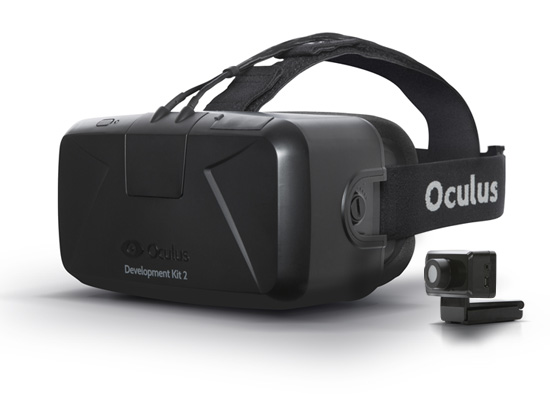
\includegraphics[width=0.6\textwidth]{Figs/oculus.jpg}
\caption{The \textit{Oculus Rift DK2} Head-Mounted Display and position tracking camera \cite{Parisi15}.}
\label{fig:oculus}
\end{figure}
\textit{DK2} was released in 2014 as the successor of \textit{DK1}, with better resolution (1920 x 1080 pixels, 960 x 1080 per eye) and positional tracker, which was not introduced in a previous model. Therefore, it enables the user not only to look around, but also to move around a virtual scene.  For the head tracking purposes, \textit{Rift} combines inertial and magnetic tracking in so-called Inertial Measurement Unit (IMU) what results in a 3 DOF effect. 6 degrees of freedom are introduced by optical tracking, with usage of micro-LED markers on the headset and IR camera. Although this solution improves immersion effect, it is still not perfect, as the user needs to be in front of the tracking camera, what limits his area of movement. This issue is  going to be solved soon with introducing third generation of \textit{Oculus}, called \textit{Crescent Bay}, which has 360-degree head tracking and higher resolution of an image. 

What is more, \textit{Oculus} producer provides needed software, \textit{Oculus Runtime} and \textit{Software Development Kit} (SDK) for developers sake \cite{Parisi15, Oculus16}. Additional facilitation constitutes availability of engines that are strongly focused on developing applications for \textit{Rift}, like Unity3D.
\subsection{\textit{Google Cardboard}}
Introduced in 2014, \textit{Cardboard VR} hastens Virtual Reality experience possibility for an average consumer. Since it makes use of almost every smart phone (which are owned by a large part of society nowadays), it allows to immerse into VE without expensive hardware- neither HMD nor computer. \textit{Google Cardboard} is simply a box with two lenses, which should be set by a  user (Figure \ref{fig:cardboard}). 
\begin{figure}[h] 
\centering    
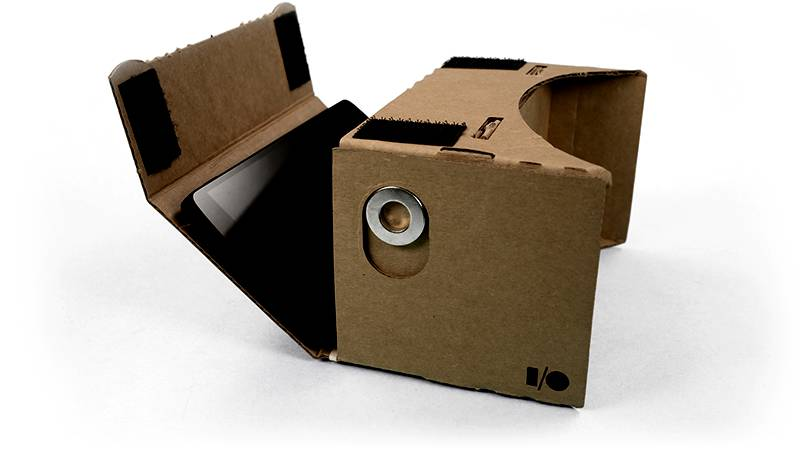
\includegraphics[width=0.6\textwidth]{Figs/cardboard.jpg}
\caption{The \textit{Google Carboard} VR viewer \cite{Parisi15}.}
\label{fig:cardboard}
\end{figure}
The stereoscopic image is created through the Cardboard-ready application on the phone, which should be placed inside the device. It provides 90° FOV and head tracking, which is generated by the phone's accelerometer and compass. Obviously, impression of immersion in this case is much smaller than in previously described device, but availability of this solution makes it more and more popular. In number of applications as well- hundreds of them are already accessible.

Similarly to \textit{Oculus Rift}, software for developers is also provided in this case by a producer. It exists in two options- an Android SDK and an add-in to, already mentioned, Unity3D engine \cite{Parisi15}.

\subsection{\textit{Leap Motion}}
\label{leapmotion}

Although it is not a Head-Mounted Display, like the previous examples, \textit{Leap Motion} provides user's input tool which is suitable for VR purposes. As this example of sensor device plays the key role in this work, it is described here as the only one of its kind.

Presented controller is a small peripheral USB device that uses two CCD IR cameras and three LED emitters, which generate IR light.  It tracks the position of predefined objects like palm and its finger tips in Cartesian space, relatively to to the center point of the device, which is placed at the position of the central IR emitter \cite{Weichert13}. Due to the difference in positions in which the controller may be used, it is worth mentioning that it employs right-handed Cartesian coordinate system, which is shown in Figure \ref{fig:leapCoordinates}.

\begin{figure}[h] 
\centering    
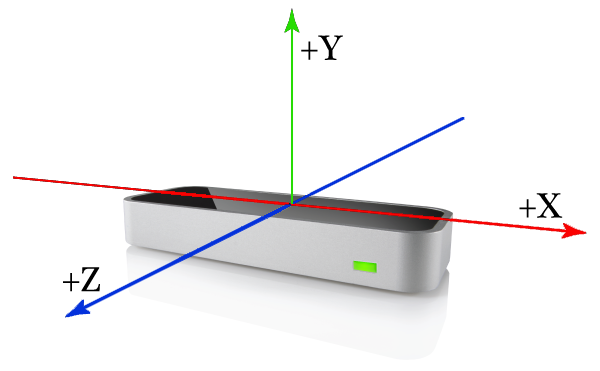
\includegraphics[width=0.6\textwidth]{Figs/leapCoordinates.png}
\caption{\textit{Leap Motion} controller and its coordinate system \cite{Leap16}.}
\label{fig:leapCoordinates}
\end{figure}

 According to the manufacturer data, the accuracy of the sensor in detection of fingertip position is approximately 0.01 mm, and the cameras frame rate varies from 20 to 200 fps depending on the user's settings and available computing power. \textit{Leap Motion} may be placed on a physical desktop or mounted onto Virtual Reality HMD. Its field of view is stated as 150° with a volume of approximately 0.23 cubic meters and the effective range varies between 25 and 600 mm above or before the device. 

 
\begin{figure}[h] 
\centering    
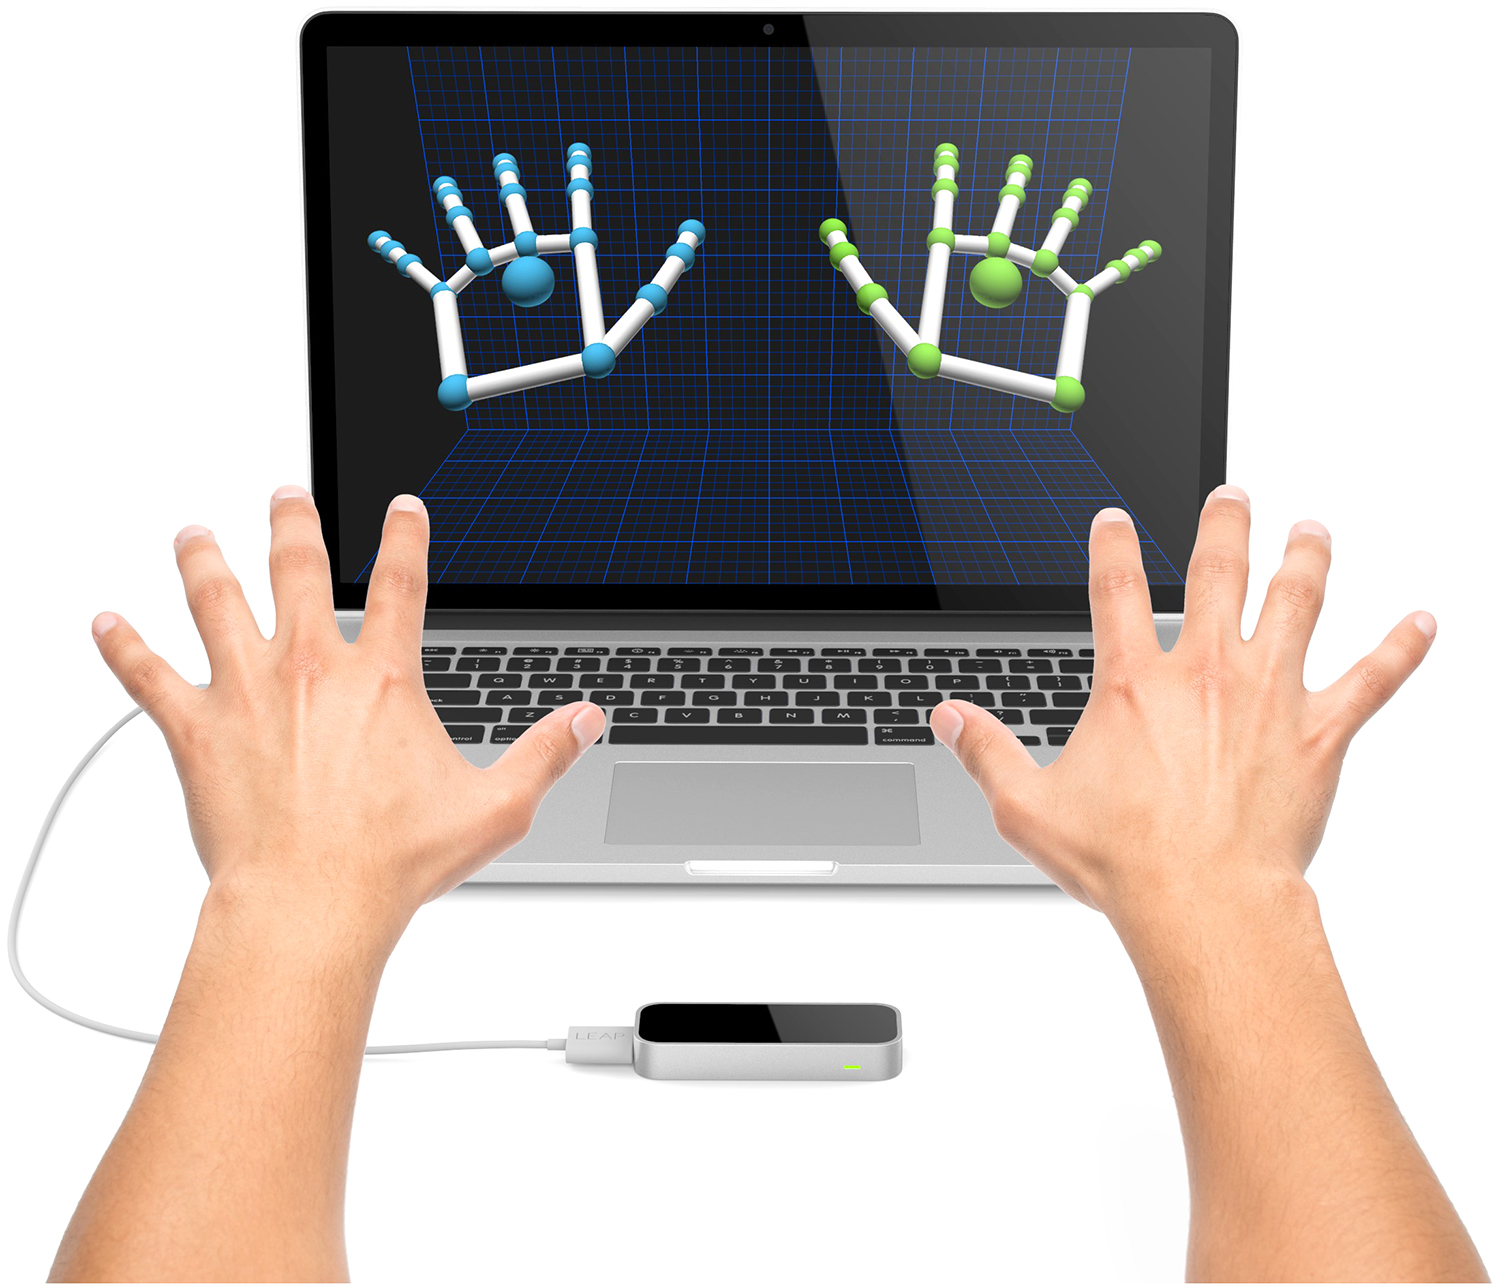
\includegraphics[width=0.4\textwidth]{Figs/leapmotion.jpg}
\caption{\textit{Leap Motion} in use- hand models on the screen are corresponding with the tracked real hands of the user \cite{Leap16}.}
\label{fig:leapmotion}
\end{figure}

The \textit{Leap Motion} API (Application Programming Interface) measures distance, time, speed and angle of the objects recorded by cameras. The software uses an internal model of human hand, what enables predictive tracking in case of temporary visibility disturbances. Moreover, the model contains all anatomical finger bones. Thanks to that, visualisation of hands in the three-dimensional VR scene is more immersive, as the model's movements are very close to its real equivalent (Figure \ref{fig:leapmotion}).
The most recent hand tracking software release, called \textit{Orion} indicates variety of improvements, dedicated mostly for VR purposes. Additionally, for the developer's use, \textit{Leap Motion} offers its SDK with libraries needed for the application development. It is available in several languages and enables integration with Unity3D engine.

%********************************** % Fifth Section  *************************************
\section{Possible applications}%Section - 1.5 
There is a large variety of applications in which Virtual Reality is and may be involved. List of possibilities constantly grows with the VE development, where entertainment constitutes the group of one of the strongest commercial potential. Therefore, many developer tools are mainly focused on creating video games, which may become more and more involving thanks to or because of VR. What is more, it creates a new way of thinking about social media and web browsing. The same happens to live entertainment- some of the famous artists have already broadcast their shows in the VE versions, making attending it possible to larger group of fans. 

But not only amusement makes Virtual Environment such an interesting and unique platform. Another industry is widely understood education. By providing interactive learning, VR may contribute to the increase of effectiveness in educating process. Thus simulations, such as medical training scenarios, scientific laboratory, flight or military reproductions, which are already created and developed, may become indispensable part of different training processes, preparing for the most unusual cases in a safe and inexpensive way. Moreover, simulations that simply create 3D VR representations may also be a valuable tool, immersing the user and facilitating understanding of presented image. That issue may be used in scientific sector, what is strongly connected with the topic of this work and described later in Chapter \ref{chapter2}. What is more, medical applications of VR are not only connected with the personnel's education. Creating the virtual world provides a platform for a new type of therapies, especially psychotherapies (like anxiety treatment) or even diagnosis, comparing reactions of possible patient with a healthy group. This topic is of great interest in a scientific world nowadays, resulting in a number of publications describing new treatment ideas.

Another field where VR is already applied is an architecture together with real estate. Creating visualisations in three dimensional view is not only a feature for designers purposes, but most of all to customers. They may experience their presence in presented properties quickly and easy, both by watching projects or video presenting already existing places. This function is also used in tourism, where showing hotel room or aeroplane interior in VR may be important for the sale success. Additionally, for those who cannot travel, VE may offer tours without getting out from their home. \cite{Parisi15, Singal15}


Examples presented here are just a few of the many other possibilities, that are constantly created. In all of them Virtual Reality facilitates or even enables humans life, and with the growing availability of VE gear it soon may become part of their every-day reality.

%makeindex <filename>.nlo -s nomencl.ist -o <filename>.nls
\nomenclature[z-API]{API}{Application Programming Interface}
\nomenclature[z-AR]{AR}{Augmented Reality}
\nomenclature[z-AV]{AV}{Augmented Virtuality}
\nomenclature[z-CPU]{CPU}{Central Processing Unit}
\nomenclature[z-DOF]{DOF}{Degree of Freedom}
\nomenclature[z-EOG]{EOG}{Electro-Oculography}
\nomenclature[z-FOV]{FOV}{Field of View}
\nomenclature[z-GPU]{GPU}{Graphics Processing Unit}
\nomenclature[z-HMD]{HMD}{Head-Mounted Display}
\nomenclature[z-IDE]{IDE}{Integrated Development Environment}
\nomenclature[z-IMU]{IMU}{Inertial Measurement Unit}
\nomenclature[z-IR]{IR}{Infrared}
\nomenclature[z-LOD]{LOD}{Level of Detail}
\nomenclature[z-MR]{MR}{Mixed Reality}
\nomenclature[z-RE]{RE}{Real Environment}
\nomenclature[z-SDK]{SDK}{Software Development Kit}
\nomenclature[z-VE]{VE}{Virtual Environment}
\nomenclature[z-VR]{VR}{Virtual Reality}
\nomenclature[z-WOW]{WOW}{Window on World}


%*******************************************************************************
%*********************************** Second Chapter *****************************
%*******************************************************************************

\chapter{Visualisation of Molecular Structures}\label{chapter2}  %Title of the First Chapter
Modern biotechnology, and thus biochemistry, genetics, molecular biology and bioinformatics as well, is based on understanding the mechanisms of molecular actions. Therefore, one of the most important information needed is a structure of molecules, such as proteins, nucleic acids, lipid layers etc. What is important to stress, is that in case of biological molecules not only general sequence is of great interest. Sequence of amino acids, in example, gives one only information about primary structure of proteins. What is meaningful as well, is their secondary (forming of $\alpha$-helices, $\beta$-sheets and turns), tertiary (spatial structure) and quaternary structure (combination of several protein chains), as those features enable protein molecules to perform their various tasks. Generally, these data make simulations and biomolecular engineering possible, enabling explaining of biological phenomena and creating new ways of influencing them.
%********************************** %First Section  **************************************
\section{Biomolecular Structure Determination} %Section - 2.1 
To create the simulation of biomolecular mechanisms, one can use structural data of certain molecules, previously obtained and now collected in available data banks. Nevertheless the knowledge of techniques used to retrieve these data is useful to know their limitations and be able to choose the most adequate one. Therefore, major methods used for that purpose are listed and described below.
\subsection{X-ray crystallography} %Subsection - 2.1.1
Currently, X-ray crystallography provides the most detailed atomic structures. The whole process consists of three main steps: first, obtaining and growing crystals of a pure molecule, second, placing it in a beam of X-rays, which is diffracted into a pattern of spots, and third, computer analysis and interpretation of arisen map of electron densities in the crystal lattice. The result depends mainly on quality of crystals, which affects the resolution of created image. Described method enables obtaining high-resolution data- best crystals may result in a map providing image of elements separated by less than 1 \AA. Though, in the vast majority of studies the resolution of 1.5 \AA up to 3 \AA is reached. While the resolution of 1.5 \AA enables distinguishing each atom in a structure, the 3 \AA resolution is harder in interpretation and usually requires additional knowledge of covalent structure of the given molecule. In these cases the biggest difficulty state mobile areas of a molecule and regions on its surface, and thus the interpretation is not unambiguous. To indicate the level of trust of the result, one introduced temperature factors, known also as B-values, which provide information about the disorder of atomic positions. B-values control the shape of Gaussian distribution, which is used for describing model atoms around an atomic center. Therefore, value of temperature factor, which is equal to 10 stands for an atom, which position is sharply described, whereas 30 or more indicates high disorder of the interpreted position \cite{Goodsell04}.

\begin{figure}[h] 
\centering    
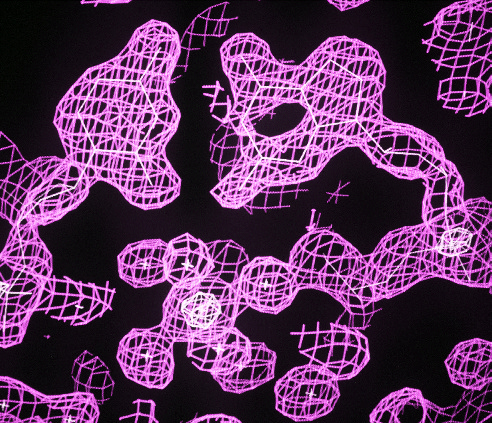
\includegraphics[width=0.5\textwidth]{Figs/xray.jpg}
\caption{Electron density map of DNA crystal \cite{Goodsell04}.}
\label{fig:xray}
\end{figure}

Besides problems with resolution, it is important to remember that the highest limitation of X-ray crystallography is simply its need of crystals, which represent one of the possible conformation, conceivably (but not necessarily) different from the one occurring in natural environment. Therefore, to overcome this issue, crystals obtained under varied conditions must be studied. This approach makes studying functional aspects of biomolecules possible.
\subsection{NMR Spectroscopy} %Subsection - 2.1.2
Another way of obtaining structural data of biomolecules is nuclear magnetic resonance (NMR) spectroscopy. It provides information about local environment of atomic nuclei. It is possible thanks to the fact, that atomic nuclei have magnetic moment, which may be aligned in a strong magnetic field. This state may be disrupted by a radio frequency pulse, which exhibits proper wavelength. What actually is measured by a spectroscopy, is the radio frequency radiation which occurs during relaxation of atomic nuclei to the basic state. It is strongly influenced by a local environment of the atom, therefore obtained data gives an information about distances between atomic nuclei and their local conformation. Usually, atomic model is developed by using a list of constraints concerning pairs of atomic neighbours and bonds between them. Its interpretation results in an ensemble of structures, which may represent all possible conformations that molecule might adopt freely in a solution or the whole range of conformations, where only one describes the actual model. In case of proteins, they differ mostly in side chains, retaining main protein chain structure.

Huge advantage of NMR technique is its applicability for molecules in a water environment, what is convenient while determining structure of biomolecules. Nevertheless, NMR spectroscopy may be used only for small proteins and nucleic acids. Even improvements in this method, such as usage of multiple radio frequency pulses which perturb multiple nuclei, enables to characterize the structure of a protein with a maximum length of 250 amino acids \cite{Goodsell04}.
 
\subsection{Electron Microscopy} %Subsection - 2.1.3
Electron microscopy methods state the approach that is the most intuitive. Nevertheless it allows to observe instead of single atoms in a molecule, only its general morphology. This issue arises from practical problems that occur while applying the technique, like imperfections of optics, problems with specimen preparations and low contrast. Therefore, the exhibited resolution is not higher than 2 nm. However, electron microscopy is often applied combined with other methods, like X-ray crystallography, NMR spectroscopy or molecular modelling. It is extremely useful not only in case of large molecules, but also to observe changes of biomolecules in different conditions. 
	\subsubsection{Transmission Electron Microscopy} %Subsection - 2.1.3.1
Transmission electron microscopy consists in illumination of a thin sample by the electron beam, whereas the microscope resolves the relative transparency of specimen regions. This method allows even to obtain a three-dimensional image by tilting the sample at a range of angles and combining resulting images (so-called electron tomography). Though, the technique is not perfect and additional proceedings are needed to improve contrast. One of them is staining the specimen with salts of heavy metals, what on the other hand may introduce artifacts. To counteract it, one may freeze the sample (cryoelectron microscopy), but it brings new problems with contrast. Thus, commonly applied approach is analysing and averaging of separate particles, which merged together give an image of whole molecule with good contrast.
	\subsubsection{Scanning Electron Microscopy} %Subsection - 2.1.3.2
Scanning electron microscopy slightly differs from its predecessor. In this approach, sample is fixed and dried and then coated with a thin metal (often golden) layer. Thereafter it is scanned with a narrow electron beam, which are scattered or emitted from a surface. This process results in a 3D image, but with relatively low resolution of 10 nm, introduced by the metal coat. Nevertheless it still may be used in research of large assemblies of biomolecules \cite{Goodsell04}.
\subsection{Atomic Force Microscopy} %Subsection - 2.1.4
The last method of determining biomolecular structures is the atomic force microscopy. It results in a topographic map of a surface of the molecule. Sample is moved under a tip both laterally and vertically (what is controlled by piezoscanners) applying a constant force on a tip. Detection of forces between specimen and cantilever is done by illuminating a laser beam on its back. Occurring reflection in different places is then caught by photo-diodes. Moreover, to reduce high shear forces that arise between tip and a sample and to prevent the latter one, the tip works in a tapping mode. Thanks to that oscillating movement, contact is shortened what minimizes shear forces. Additionally, the whole apparatus is placed in a solvent, what enables mimicking biological, natural environment and therefore give the real structure of biomolecules.

Atomic force microscopy is a really accurate tool. Its resolution depends on the sharpness of a tip, though usually is in the range between 0.1 and 10 nm. What is more, it may be applied for measuring forces between molecules or even forces that conduct protein folding \cite{Goodsell04}.
\subsection{Databases} %? %Subsection - 2.1.5
There are many kinds of bioinformatical databases, providing information about nucleotide and protein sequences, protein families, structures, their functional annotation etc. For this work the most important type constitute structural databases, therefore they are shortly described in this section.


\subsubsection{PDB}
Protein Data Bank (PDB) database was established in 1971 in USA as the tool needed for crystallographers to freely exchange protein structures between laboratories. Nowadays PDB constitutes the greatest collection of spatial structures of proteins in the world, especially since 2003, when it has been united with European Macromolecular Structure Database and PDB Japan. 

In the described database one can find structures obtained with a large variety of methods, mainly by X-ray crystallography, NMR spectroscopy and electron microscopy, which were described earlier. Before publishing of the results sent by laboratories, structure is checked for correctness and data format. Data may be presented in three kinds of files: PDB, mmCIF (macromolecular Crystallographic Information File) and PDBML (Protein Data Bank Markup Language). In the end, the structure is tagged and becomes its unique identity number. 

It is worth mentioning  the details of PDB data format, as it is mainly used by visualisation software. First of all, those files  employ so-called method of chemical rules in generating bonds between atoms. Practically, it means that there is a need of tables with types and typical lengths of bonds between certain atoms. Thanks to that, for example, if two carbon atoms are 1.5 {\AA} apart, it is assumed that they are bonded with single bond and thus the amount of information in one file is reduced. On the other hand, this solution is problematic in unusual cases, when such estimations are incorrect. What is more, data in the PDB files is divided into two groups. First one, explicit sequence, is marked with the lines with a SEQURES symbol, where one can find sequence of amino acids in certain chain of protein. However, to reconstruct the whole structure it is not enough, therefore implicit sequence is needed. In this type every single atom is represented separately with its position in Cartesian coordinate system in the space (x, y, z), its name, number in the structure, the number of the residue that atom belongs to, number of possible conformations etc. Those lines are assigned with an ATOM (usually for atoms belonging to nucleic acids or proteins) or HETATM (for small molecules) symbol \citep{Gruca10}. The whole format description and the contents guide is found on the website of Worldwide Protein Data Bank.

\subsubsection{MMDB}
Molecular Modelling Database (MMDB) which belongs to National Center for Biotechnology Information (NCBI) is strictly connected with the PDB structures, but it is extended with Entrez system, which enables the access to all biological data concerning the molecule. In this case, PDB file is translated to the ASN.1 (Abstract Syntax Notation) format, where one can additionaly find such information as unified definition of secondary structure or the spatial domain structure. In contrast to PDB files, ASN.1 contains data about every bond specifying its category (explicit bonding approach). Nevertheless it uses so-called dictionary of the residues, where atoms and bond of 20 amino acids and 8 nucleotide groups are described \citep{Gruca10}.

%********************************** %Second Section  *************************************
\section{Representation of Structures with Computer Graphics}   %Section - 2.2 
To explore and understand the working mechanisms of biomolecules, the already known structure needs to be visualized. Obviously, direct imaging in this case is impossible, as molecules are significantly smaller than the wavelength of visible light. To overcome this issue, a large variety of representations have been developed and are useful for different purposes. All of them should have two things in common: clarity - being understandable for the user and maintaining the properties of a molecule that are directly related to the nano-scale world. Here, a few most popular ones are described.

\begin{figure}[h] 
\centering    
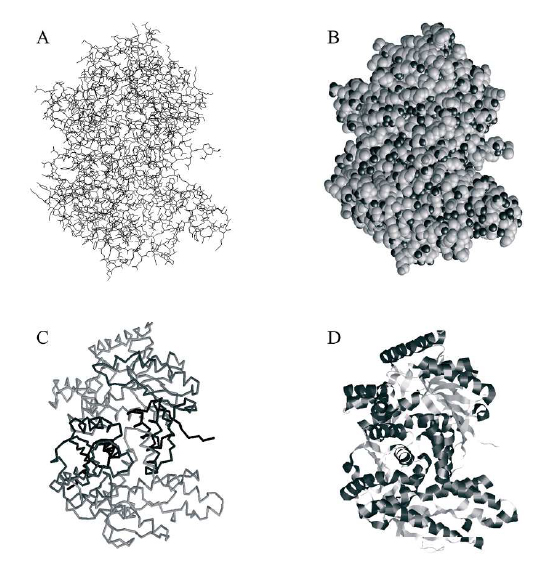
\includegraphics[width=0.8\textwidth]{Figs/visualization.jpg}
\caption{Lactate dehydrogenase presented in four ways: A- wireframe (bond diagram), B- spacefilling, C- backbone (ribbon), D- secondary structure (cartoon) diagram \cite{Gruca10}.}
\label{fig:visualization}
\end{figure}

First one, which is so-called "Ball-and-Stick" representation is the most fundamental one, presenting atoms as "balls" and bonds between them as "sticks". Although this approach is typical for education purposes, it does not provide relevant information. Most of all, it is misleading in case of the volume that molecule occupies, as the spheres are smaller than atomic radii to obtain the clearer view. Certainly, bonds presented as sticks give a comprehensive image for the user, nevertheless it is distant from the reality.  
Secondly, wireframe diagram (Figure \ref{fig:visualization} A) is simply representation of covalent bonds between atoms, presenting them as lines. It gives, similarly to "Ball-and Stick" approach, a view for the geometry of a whole molecule and finds an application in investigating linkings of proteins with cofactors or structures of active sites. On the other hand, spacefilling view (Figure \ref{fig:visualization} B) represents each atom as the relative sphere (for example Van der Waals sphere). This approach is the most relevant for size and shape representation, what is needed for visualisation of interactions between molecules. Then, ribbon diagram (known also as backbone) shows the topology of protein chain to the user and it is based on linkings between $\alpha$-carbons of each amino acid. The last representation, called "cartoon" is focused on the secondary structure of the protein, presenting $\alpha$-helices as twisted ribbons and $\beta$-sheets as arrows. Those two last examples (Figure \ref{fig:visualisation} C and D) are commonly used for topology, protein folding analysis and its comparison between different molecules \citep{Goodsell04, Gruca10}. 

Modern software used for visualisation is able to read the structural data and image it in a way that user needs. Obviously, to fulfil their task and be useful for users, such programs need to make rotation and zooming of the models possible. Moreover, additional features are helpful, such as measurements of distances and angles between atoms, identification of certain features of the structure and colouring, which significantly increases clarity of presented view. Generally user may choose from a large collection of colouring systems. In example, CPK, where each type of atom is coloured differently (carbon- grey, oxygen- red, hydrogen- white, nitrogen- blue etc.), shapely colouring, where each amino acid or nucleotide has got a different shade, chain, which, instinctively, differentiates each chain, group, where C- and N- or 3' and 5' ends are coloured differently, temperature, which helps to identify vibration degree of freedom for each atom etc \citep{Gruca10}. What is more, some of the software is not only visualisation tool and often provide a large engine for molecular modelling simulations, like program called VMD. On the Protein Data Bank Website, one can find a list of 41 programs used for biomolecular visualisations, some of them with open source or academic license.
 
%********************************** %Third Section  *************************************
\section{Virtual Reality in Visualisation of Structures}%Section - 2.3
Nowadays, a large amount of model organisms proteins have been researched and their structures are currently available in the data banks. This improvement coincides with the lastly observed computer processing power and memory growth. With addition of steady decrease of hardware prices, those occurrences create a great conditions for development of biomolecular visualisation, which leads to application of Virtual Reality for chemical and biological sciences.

\subsection{Motivation}
The most important investigation which should be done, is considering, whether engaging VE to bioinformatics is worth trying, and if so, what are the potential benefits from that solution. To answer these questions, it is convenient to describe issues that currently scientists have to deal with. First of all, for better understanding of proteins functions, their interactions and conformational changes should be known, and that is possible with the dynamically explored visualisation. Although classical approach results in still improving programs, it creates the 3D representation in the two-dimensional space, where depth perception and immersion is often not sufficient. Moreover, when several models are needed to be imaged at the same time, the view becomes unclear and structure manipulating becomes more difficult. Problem appears as well when small changes occur, such as in transient state interactions, which should be easily observable for better phenomena explanation. Furthermore, in the bioinformatics field, the human factor still plays an important role, for example in the structure interpretation and solving (often by comparative modeling) or in receptor docking simulations, when the algorithms cannot perform sufficient visual pattern recognition. Those subjects are highly important in drug design. For example, if the protein binding site is unknown, searching for possible sites need to be performed by experienced researcher and this case requires as best graphical representation of a structure as possible. Additionally, thanks to precise observations of a protein binding site, scientist may form a good hypothesis for ligand design, what is one of the most interesting tasks of molecular modelling \citep{Anderson99}. 

Those issues can be overcome or at least become easier thanks to Virtual Reality, due to its immersion effect, its intuitiveness and possibility of real-time visualisations creation. Three-dimensional image enables direct manipulation of models and interactions between them. It facilitates observation from different points, looking around and distinguishing of each structure. Although this idea does not mimic any known real surrounding, it creates an exact representation of nano-reality and enables discovering its features. Molecular modelling, molecular dynamics and bionanotechnology tools may be implemented in VR environment, creating a powerful combination that facilitates a large variety of bioinformatics tasks.  

\subsection{Examples}

The idea of combining Virtual Environment with biomolecular simulation is not new. Already described in Chapter \ref{chapter1}, \textit{GROPE} and CAVE systems were used for those purposes in 1990s. Both were applied to drug-enzyme docking procedure, while the latter was a visualisation system, which actually had its input in discovery of new molecular features. Nevertheless, it was really expensive and, what is more disturbing, it did not give the user a reference point where he or she is in the virtual world. It hinders image manipulation and gives user a feeling of disorientation \citep{Mazuryk96, Schulze11}. Then, in 2000, Abraham Anderson and Zhiping Weng created program called \textit{VRDD}, which was actually a drafting table-style projection system with additional wand with buttons, which was a program controller and remote. Additionally, the concept allowed to use a keyboard for more complex tasks. \textit{VRDD} could present different display models, enabled docking simulations, real-time calculation of binding free energies and searching for binding sites by restricting it to possible regions \citep{Anderson99}. Next, the very specific tools for VR were made, like the one designed for nucleic acids only, which can create long chains and therefore generate huge amount of data \citep{Herisson05}, or one for bionanorobotics prototyping, which main task was to invent protein-based molecular machines with usage of molecular dynamics methods \citep{Hamdi08}.

The last example constitutes \textit{Molecular Rift}, the program implemented in 2015 for \textit{Oculus Rift} by Magnus Norrby et al. What is more, it makes use of \textit{MS Kinect} gaming sensor for gesture steering, which has its equivalents in keyboard steering as well. \textit{Molecular Rift} is able to read three structure file formats: PDB, MOL2 and SDF and to perform calculations with several forcefields thanks to usage of \textit{Open Babel} chemical tool kit, make representations in different styles and colours and label specific atoms or amino acids. Additionally, the authors made user tests, which encourage to further improvements, as, despite some minor problems, the tool was rated as useful and interesting by the group of scientists \citep{Norrby15}. 

\subsection{Problems and future}

Despite all the advantages of VR application to bioinformatics, it also generates difficulties, which need to be overcome to make it a standard technology in molecular visualisation. Performance limitations constitute one of them. Complexity of the vast majority of biomolecules generates high computational cost if visualized, increasing the demand for CPU and GPU processing power of the computer. Although technological development causes new solutions that provide better efficiency of computers, the overall performance may be improved on the software site as well. In example, developers of \textit{ADN-Viewer}, program dedicated for nucleic acids imaging, implemented the idea of decrease of image quality with the distance from the user. It means, that the closest objects were represented in great details, whereas further ones- with lower accuracy. Moreover, they applied algorithm that deletes currently hidden parts of the structure from the data, what saves computational expenses \citep{Anderson99}. 

Next problem that occurs while developing for VE is the issue of navigating tools, which are necessary for the proper exploration of biological structures. In three-dimensional space it is problematic to place 2D control panel. What is more, as currently most common gear for VR is a Head-Mounted Display, which is not transparent, limitations of external input devices (mouse, keyboard, joysticks) usage occur. Nevertheless this difficulty decreases, thanks to new possibilities that appear on the market, like VR gloves, eye-tracking devices, cameras etc. However, need of such specialised equipment generates additional costs. Anyway, the rule which need to be followed is that the program should be made in a way that minimizes the possibility of user disorientation \citep{Anderson99, Norrby15}.

It is important to remember, that creating visualisation programs for VE requires cooperation of programmers and biologists, to make it as effective and useful as possible. Although there is still no software available commercially for described purposes, many papers reports new solutions in this topic, what indicates the need of visualisation improvement. Nowadays, biotechnology development and the speed of this development is strongly dependent from bioinformatics, thus one can conclude, that the potential market is relatively large. Additionally, next step in this issue for the future development is the visualisation of whole cells or even biological pathways and organelles, as Norby et al. suggest the idea of such representations, with the function of simulating and steering the biological regulation. Furthermore, it should be stressed out that scientific usefulness of VR is followed by educational one. Understanding the contents of big data largely depends on the way it is presented. Surely "gamification" and interactiveness of biochemistry could make it more attractive and assimilable for students, what may happen to be a good investment in science in the future \citep{Norrby15}.  
%makeindex <filename>.nlo -s nomencl.ist -o <filename>.nls
\nomenclature[z-mmCIF]{mmCIF}{macromolecular Crystallographic Information File}
\nomenclature[z-MMDB]{MMDB}{Molecular Modelling Database}
\nomenclature[z-NCBI]{NCBI}{National Center for Biotechnology Information}
\nomenclature[z-NMR]{NMR}{Nuclear Magnetic Resonance}
\nomenclature[z-PDB]{PDB}{Protein Data Bank}
\nomenclature[z-PDBML]{PDBML}{Protein Data Bank Markup Language}


%*******************************************************************************
%*********************************** Third Chapter *****************************
%*******************************************************************************

\chapter{Molecule VR Viewer}\label{chapter3}  %Title of the Third Chapter

This chapter describes all functionalities of the core and, simultaneously, result of presented work, which is the Molecule VR Viewer program. Description of methodology and implementation details are discussed in Chapter \ref{chapter4}.

Generally, Molecule VR Viewer is an application that presents structure of the molecule in Virtual Reality, basing on the data contained in PDB file. As the program provides several modes and options, functionalities are described step by step, starting from the main menu. For its full performance, application requires \textit{Oculus Rift} HMD with attached \textit{Leap Motion} device. 

%********************************** %First Section  **************************************
\section{Main Menu} %Section - 3.1 

As main menu window is created in 2D and requires keyboard and mouse input, it is not rendered for \textit{Oculus}. Starting panel is presented in Figure \ref{fig:mainmenu}.

\begin{figure}[h]
\centering    
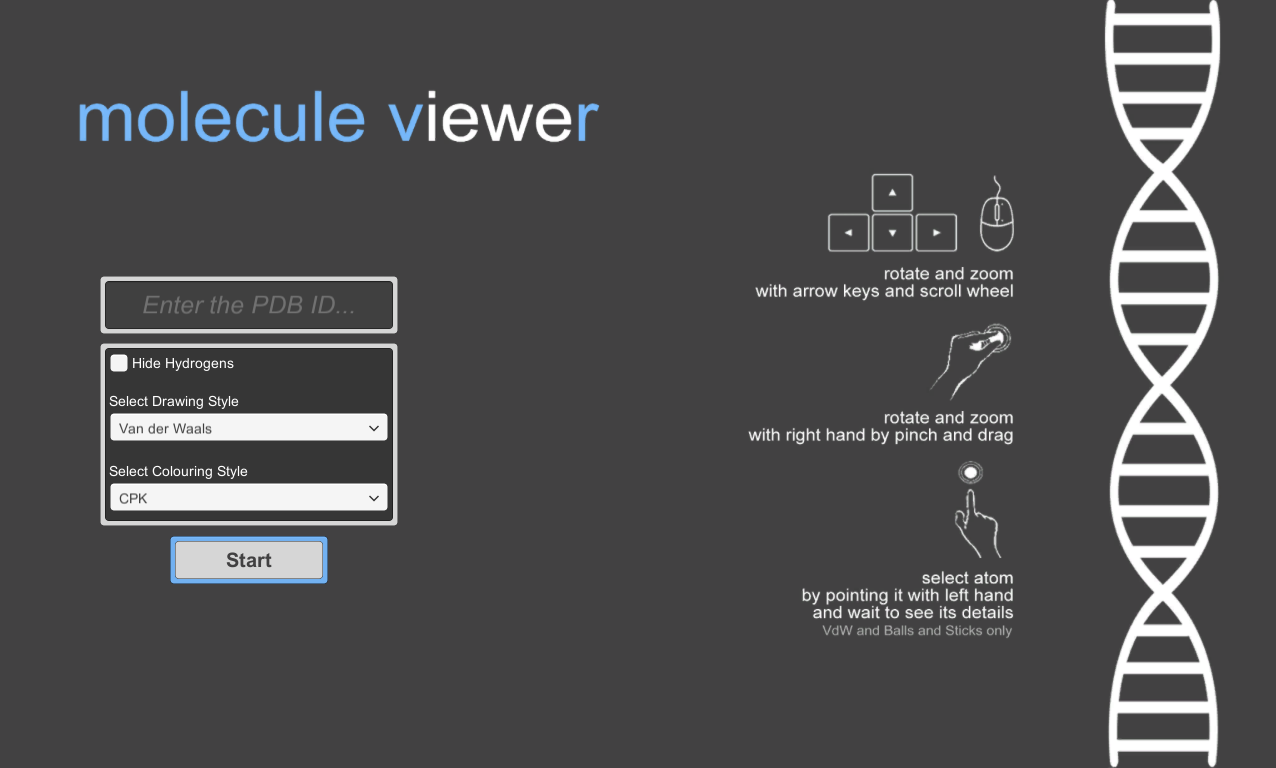
\includegraphics[width=1.0\textwidth]{Figs/mainmenu.png}
\caption{Starting window of the Molecule VR Viewer program.}
\label{fig:mainmenu} 
\end{figure} 

In the first input field, user is asked to enter the PDB ID- the four-character unique code that stands for a single molecule structure, which may be found in Protein Data Bank. Next, in settings panel, user may influence three properties of the generated visualisation. Toggle box "Hide Hydrogens" enables to choose whether to take hydrogen atoms into account while generating the structure or not. This function is purely practical, as the big number of hydrogen atoms (which often constitute around 50\% of the protein) may affect clarity of the view. However, if the PDB file does not provide data about hydrogen atoms (due to the method of obtaining the structure), toggle does not have any influence on the created view. Then, user may choose drawing and colouring style from the two drop down lists, but the choice of the representation style affects on the availability of colouring methods- for each drawing method different colouring settings may be applied. Application provides five different drawing settings: Van der Waals, Lines, Balls and Sticks, Ribbon and Backbone and four colouring styles: CPK, Residues, Subunits ans Secondary Structures. All of them are described in the following subsections.

On the right side of the menu window, short user's guide with pictograms presents the ways of rotating ad zooming the view, switching between modes and how to use the pointing mode.   

After clicking the "Start" button, correctness of the entered PDB ID is checked. In case of problems, error message occurs, allowing the user to recognize the problem. If the PDB code was found in the database, program presents "Wait..." message and analyses the selected structure to draw it. From this moment, user may put on the head-mounted display.
   
%********************************** %Second Section  **************************************
\section{Drawing Styles} %Section - 3.2

\subsection{Van der Waals}

Van der Waals representation creates for each atom a sphere of Van der Waals radius, which is different for every single element. It illustrates the imaginary volume that is occupied by the atom, in which it may interact with other atoms. When the atoms are bounded covalently, their Van der Waals spheres overlap. Thus, the representation shows the approximate shape of the whole molecule and its potentially accessible places, like active sites, which are highly important in case of ligands binding, their design etc. Example of such shape obtained with Molecule VR Viewer is shown in Figure \ref{fig:vdw}.

In addition to CPK colouring style presented in the example, Van der Waals drawing style enables Residues and Subunits colouring. 

\begin{figure}[!htb]
\centering    
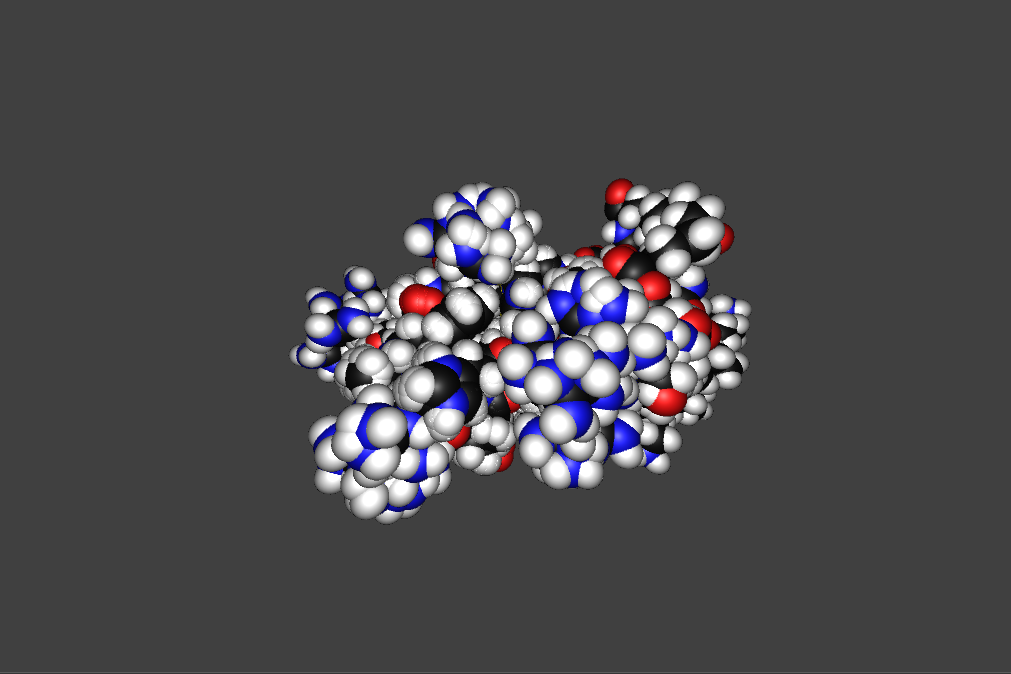
\includegraphics[width=0.8\textwidth]{Figs/vdw.png}
\caption{Van der Waals representation of yeast transcription factor ADR1 (PDB ID: 1ARD) with CPK colouring and showed hydrogens.}
\label{fig:vdw} 
\end{figure}

\subsection{Lines}
\begin{figure}[!htb]
\centering    
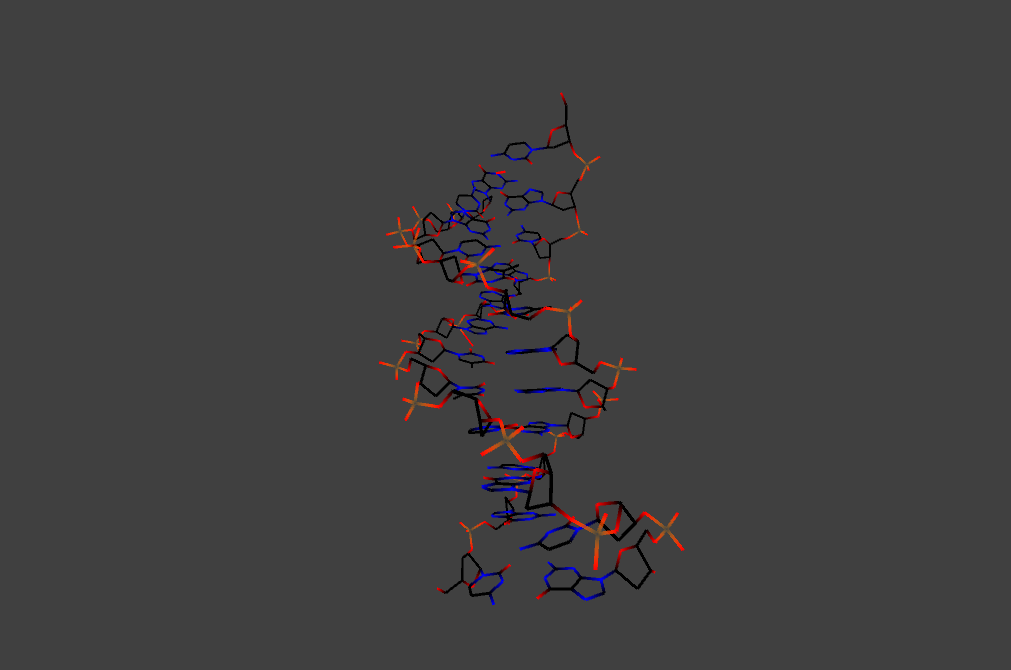
\includegraphics[width=0.8\textwidth]{Figs/lines.png}
\caption{Structure of the B-DNA dodecamer (PDB ID: 1BNA) obtained with Lines style and CPK colouring. The double helix structure of this nucleic acid is clearly visible, as well as belonging nucleobases.}
\label{fig:lines} 
\end{figure}

Another visualisation style is showing the covalent bonds existing in the structure and because of that is called Lines representation. Resulted wireframe is clear and, for the experienced scientist, easy to understand and to distinguish individual residues. Comparing to Van der Waals representation, Lines show the skeleton of the molecule, resulting in not crowded view, where one can easily find, for example, chemical rings. The exemplary structure made with bond diagram is presented in Figure  \ref{fig:lines}.

As shown, CPK colouring in this representation is made by smooth transition of colour between bonded atoms. The colouring options in this case are same as in Van der Waals setting.

\subsection{Balls and Sticks}

\begin{figure}[!htb]
\centering    
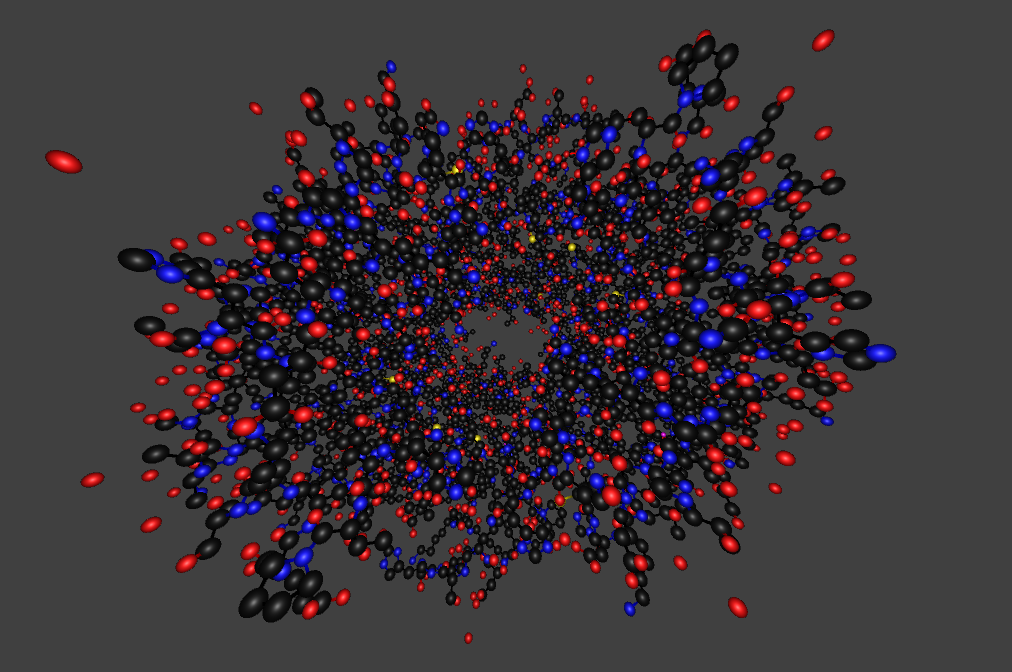
\includegraphics[width=0.8\textwidth]{Figs/balls.png}
\caption{Deoxy human hemoglobin (PDB ID: 1A3N) - important transporter of oxygen, shown with Balls and Sticks setting and CPK Colouring.}
\label{fig:balls} 
\end{figure}

Balls and Sticks is simply fusion of Lines and Van der Waals representation. To make the clear view, radii of the atoms are twice reduced. This drawing style is widely used in the molecule visualisation for better understanding, especially for education purposes. Nevertheless it is important to remember, that real atoms are not spheres bonded with sticks, and such idea is only a convention, which does not provide proper information about molecular shape. Illustration of Balls and Sticks representation demonstrates Figure \ref{fig:balls}. As the presented example is constituted by relatively big protein (tetramer- consists of four chains), the general view seems to be unclear. This case proves, that magnifying the view and looking around freely is crucial in the context of useful visualisation.


\subsection{Backbone}

As protein is, generally saying, chain of amino acids, which are connected with peptide bonds, it does have a main backbone trace. It is one of the most simplified type of representation and is obtained by omitting amino acid side chains. In case of protein, the backbone is created between alpha carbon atoms (carbon atom before the carbonyl carbon in peptide, which bonds with amino acid residues). What is more, nucleic acids are biopolymers as well, and their backbone is created by phosphate and deoxyribose molecules, and in simplified form- by linked phosphorus atoms.

This representation style puts emphasis on the secondary structure, ignoring the primary one somehow. In this approach is not the single residues that matters, but the structures that they form. Additionally, this drawing setting is great for showing the tertiary structure- protein geometric shape or even quaternary one- with all the subunits of molecule, as presented in Figure \ref{fig:backbone}. Because of all those properties, the only colouring method applicable here is the Subunits style.

\begin{figure}[!htb]
\centering    
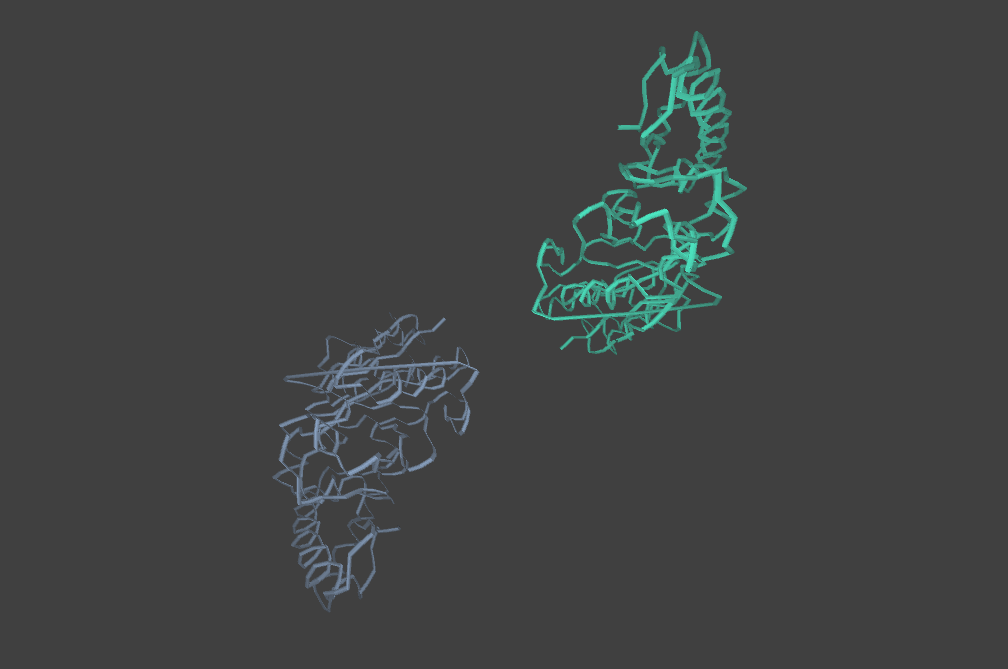
\includegraphics[width=0.8\textwidth]{Figs/backbone.png}
\caption{Papain dimer (PDB ID: 4QRV) presented in Backbone style with Subunits colouring. One can recognize alpha helix structures occurring in each chain.}
\label{fig:backbone} 
\end{figure}

\subsection{Ribbon}

The last drawing style supported by Molecule VR Viewer is Ribbon diagram. It is one of the most commonly used in both scientific and educational world, since it illustrates the whole organisation of protein structure. One can say, that it is improved Backbone representation, with even bigger emphasis put on secondary structure. It is achieved by presenting $\alpha$-helices and $\beta$-strands, the most common and important secondary structure types, as cylindrical spiral ribbons and arrows, respectively, both following the backbone of the peptide. $\beta$-sheet arrows, except just their distinguishing from other structures, play another important role- they show the direction of protein chain, from amino to the carboxyl end. These are the crucial elements of ribbon diagram and they are supported by Molecule VR Viewer, however, in more complex diagrams, other structures, such as loops, turns or even disulfide bonds may be presented. 

\begin{figure}[!htb]
\centering    
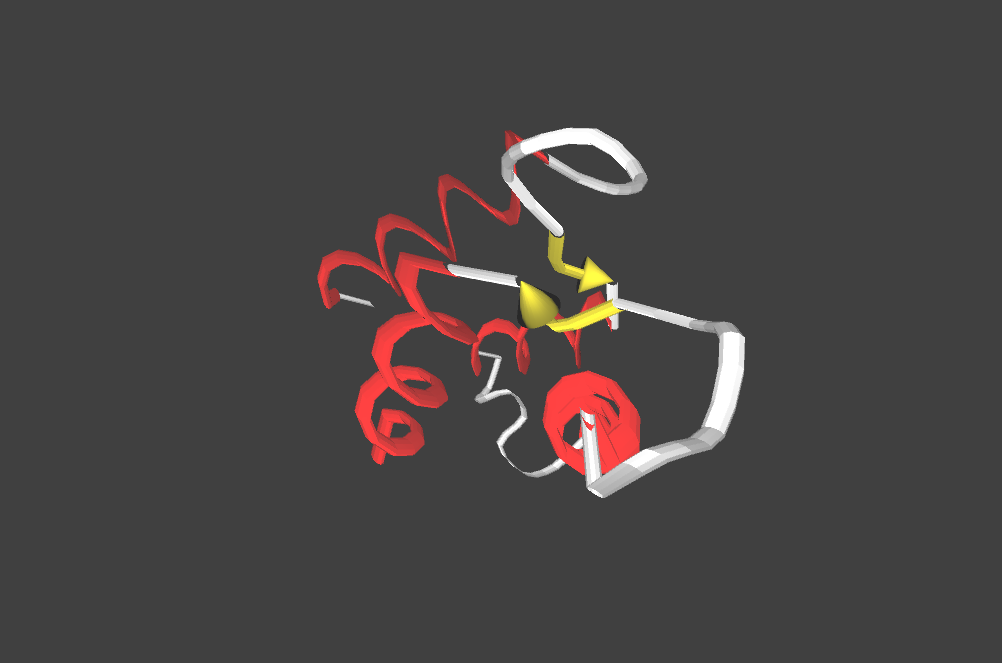
\includegraphics[width=0.8\textwidth]{Figs/ribbon.png}
\caption{Ribbon diagram of calbindin D9k from \textit{Bos Taurus} (PDB ID: 2BCA) with noticeable four $\alpha$-helices and two $\beta$-strands}
\label{fig:ribbon} 
\end{figure}

Exemplary protein visualised with Ribbon representation is shown in Figure \ref{fig:ribbon}. In this diagram the most useful colouring style was set- Secondary Structure. However, it is possible to apply Subunits colouring as well.

 


%********************************** %Third Section  **************************************
\section{Colouring styles} %Section - 3.3 
\subsection{CPK}
Colouring style called CPK from it's authors names (Corey, Pauling, Koltun) is a standard convention of colouring atoms on basis of elements they represent \cite{Koltun65}. As the original patent of Koltun does not mention all of the elements that may occur in biomolecules, they have been set for this work purposes, and the result is shown in Table \ref{tab:cpk}.

\begin{table}[h]
\centering 
\begin{tabular}{|r|c|}
  \hline 
  H & \cellcolor[rgb]{1,1,1} \\
  \hline
  C & \cellcolor[rgb]{0,0,0} \\
  \hline
  N & \cellcolor[rgb]{0,0,1} \\
  \hline
  O & \cellcolor[rgb]{1,0,0} \\
  \hline
  F, Cl & \cellcolor[rgb]{0,1,0} \\
  \hline  
  P, Fe & \cellcolor[RGB]{255, 153, 0} \\
  \hline
  S & \cellcolor[rgb]{1, 0.92, 0.016} \\
  \hline
  Br & \cellcolor[RGB]{153, 0, 0} \\
  \hline
  I & \cellcolor[RGB]{148, 0, 211} \\
  \hline
  Be, Mg, Ca, Sr, Ba, Ra & \cellcolor[RGB]{0, 102, 0} \\
  \hline
  Li, Na, K, Rb, Cs, Fr & \cellcolor[RGB]{159, 0, 255} \\
  \hline
  Ti & \cellcolor[rgb]{0.5, 0.5, 0.5} \\
   \hline
  other & \cellcolor[RGB]{255, 0, 227} \\
  \hline
\end{tabular}

\caption{CPK colour assignments used in Molecule VR Viewer.}
\label{tab:cpk}
\end{table}

The big advantage of this style is its clarity and the easiness of recognizing e.g. metal cofactors in metalloproteins. Such example is presented in the Figure \ref{fig:cpk}


\begin{figure}[!htb]
\centering    
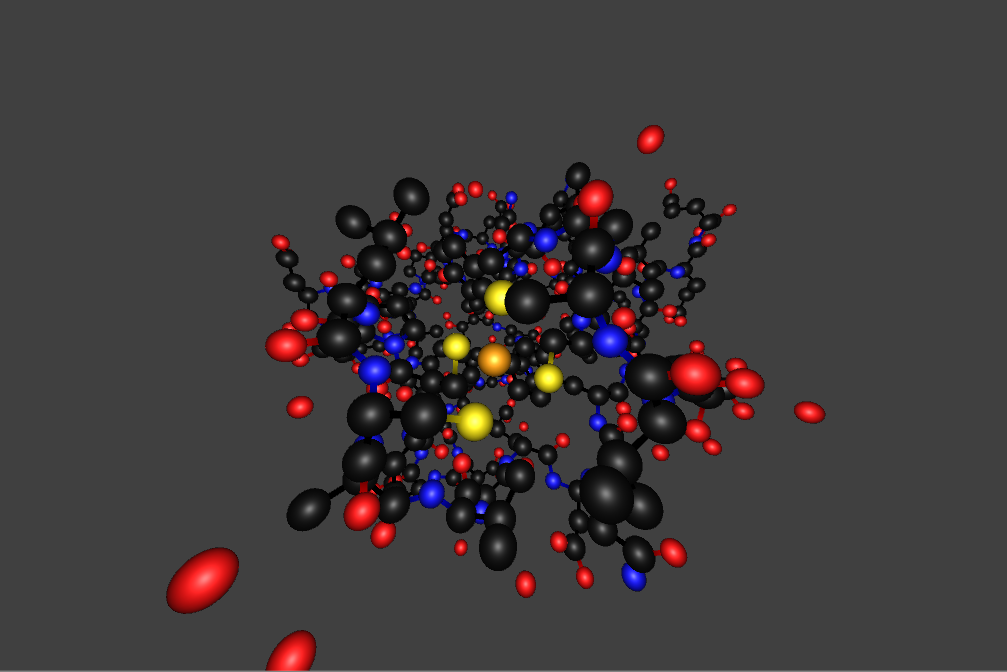
\includegraphics[width=0.8\textwidth]{Figs/cpk.png}
\caption{Fe$^{3+}$ ion (orange) in the binding pocket made out of 4 cysteine residues in the structure of rubredoxin (PDB ID: 1B2J) presented in CPK colouring mode and Balls and Sticks representation.}
\label{fig:cpk} 
\end{figure}

\subsection{Residues}

Both proteins and nucleic acid consist of meres- amino acids and nucleotides, respectively. Although, as mentioned before, experienced scientist may recognize the residue directly from its structure, it is more convenient to apply the distinguishing colouring style. Since there are 20 basic amino acids that build proteins, their colours were assigned following to the scheme presented in Table \ref{tab:residues}, which comes from the \textit{RasMol}, molecular visualisation program \cite{Rasmol16}. All of the other residue types have random color assigned. The example shows Figure \ref{fig:residues}.

\begin{table}[h]
\centering 
\begin{tabular}{|r|c|}
  \hline 
  ASP,GLU & \cellcolor[RGB]{230,10,10} \\
  \hline
   LYS,ARG & \cellcolor[RGB]{20,90,255} \\
  \hline
  PHE,TYR & \cellcolor[RGB]{50,50,170} \\
  \hline
  GLY & \cellcolor[RGB]{235,235,235} \\
  \hline
  ALA & \cellcolor[RGB]{200,200,200} \\
  \hline  
  HIS & \cellcolor[RGB]{130,130,210} \\
  \hline
  CYS, MET & \cellcolor[RGB]{230,230,0} \\
  \hline
  SER,THR & \cellcolor[RGB]{250,150,0} \\
  \hline
  ASN,GLN & \cellcolor[RGB]{0,220,220} \\
  \hline
  LEU,VAL,ILE & \cellcolor[RGB]{15,130,15} \\
  \hline
  TRP & \cellcolor[RGB]{180,90,180} \\
  \hline
  PRO & \cellcolor[RGB]{220,150,130} \\
   \hline
\end{tabular}

\caption{Amino acid colour assignments used in Molecule VR Viewer \cite{Rasmol16}.}
\label{tab:residues}
\end{table}

\begin{figure}[!htb]
\centering    
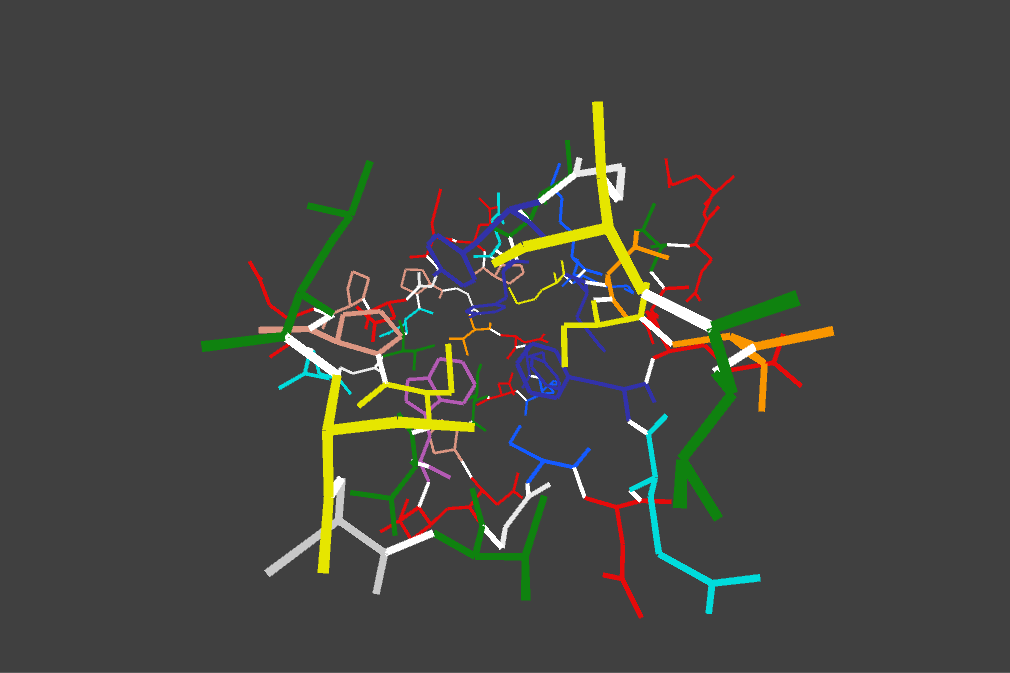
\includegraphics[width=0.8\textwidth]{Figs/residues.png}
\caption{The same rubredoxin (PDB ID: 1B2J) as in Figure \ref{fig:cpk}, presented with Residues colouring and Lines representation. In this case one can recognize 4 cysteine residues directly (yellow), not from the sulfur atoms.}
\label{fig:residues} 
\end{figure}

\subsection{Subunits}

Since protein or nucleic acid may be an assembly made of multiple chains, forming quaternary structure (in case of peptides), it is sometimes of high importance to recognize which atom belongs to which subunit, whether subunits are identical (homomers) or not (heteromers). Usually chains are named with consecutive letters of the alphabet, nevertheless, it is not a standard. Therefore, in Molecular VR Viewer, the colour of each subunit is assigned randomly, resulting in the image like in Figure \ref{fig:subunits}.

\begin{figure}[!htb]
\centering    
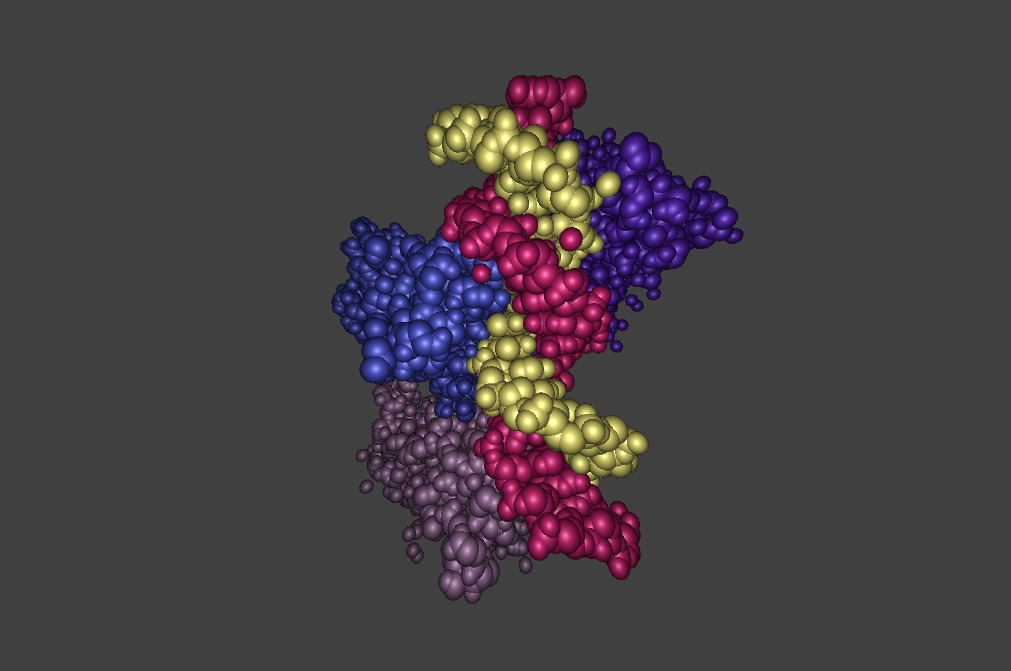
\includegraphics[width=0.8\textwidth]{Figs/subunits.png}
\caption{Tumor suppressor p53, which is of high interest in scientific world, complexed with DNA (PDB ID: 1TUP) presented with Subunits colouring and Van der Waals representation. It is not hard to distinguish two DNA chains (pink and yellow) forming double helix, from the protein units.}
\label{fig:subunits} 
\end{figure}

\subsection{Secondary Structures}
The last colouring setting, dedicated for Ribbon diagram, is the simplest one. As shown in Figure \ref{fig:ribbon}, each type of secondary structure has different colour assigned. $\alpha$-helices are red, $\beta$-sheets are yellow and the rest of the backbone is white. This style intensifies the effect of distinguishing secondary structures introduced in Ribbon drawing style.

%********************************** %Fourth Section  **************************************
\section{Visualisation Scene} %Section - 3.4

After clicking the "Start" button, required structure is loaded and user may start to watch and explore it. At the beginning, the molecule spins around its center, what may be stopped by pressing any key or what stops automatically after 15 seconds. Moreover, the name of presented molecule is displayed on the upper side of the user's view, which disappears after 15 seconds as well. With the \textit{Oculus} HMD on, user may look around this simulated nano-world.

\subsection{Rotating and Zoom}

Rotating and magnifying of the molecule is one of the most important feature for the properly designed visualization tool. In Molecule VR Viewer it may be accomplished in two ways. First one is simply pressing arrow keys on computer's keyboard for rotation up-down and left-right or scrolling the mouse wheel for zooming in and out. Nevertheless, with a head-mounted display on, user may find pressing the proper key hard, as the \textit{Oculus} headset does not provide transparency and the whole vision is covered with VR. Therefore, the second way is introduced.

Rotating and zooming of the image may be obtained by the Leap Motion Controller, the device already described in subsection \ref{leapmotion}. If it is attached to the HMD, it requires only to extend right arm forward. Then, on the viewer scene the hand model should appear, which is the exact equivalent of the user real hand.

To start moving the scene, user needs to make a pinch gesture (with index finger and thumb). Without releasing it, movement of the hand up-down and left-right rotates the molecule. For zooming in, user should pinch and pull it to yourself, for zooming out- pinch and push forward. The hand model making pinch gesture on the Molecular VR Viewer scene illustrates Figure \ref{fig:pinch}.    

\begin{figure}[!htb]
\centering    
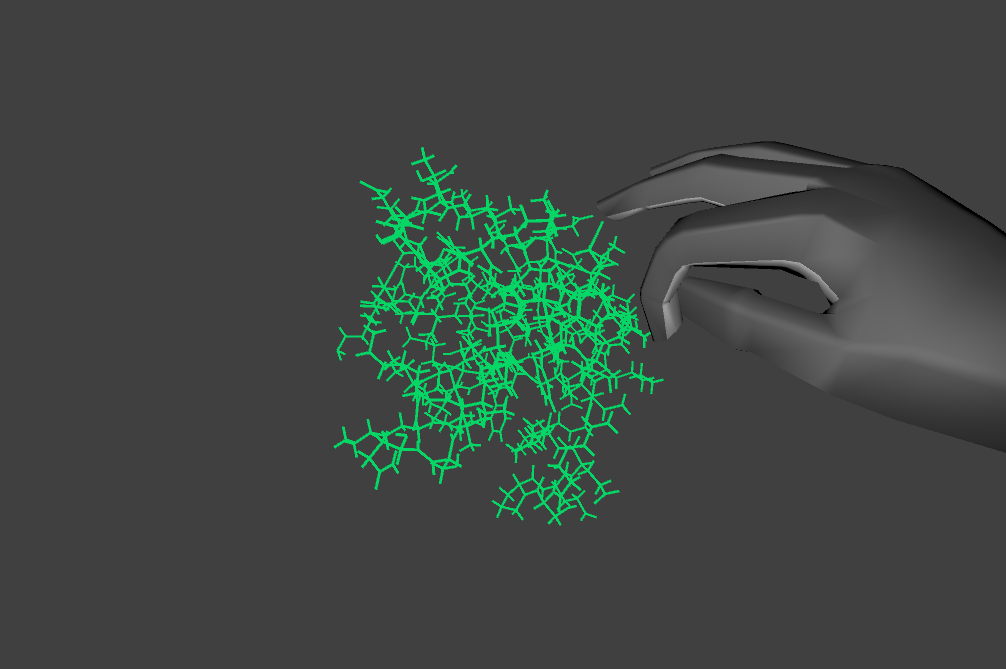
\includegraphics[width=0.8\textwidth]{Figs/pinch.png}
\caption{Pinching gesture enables rotation and magnifying of the structure.}
\label{fig:pinch} 
\end{figure}

Manipulating with \textit{Leap Motion} usage requires a bit of practice. However, this solution is perfect for the Virtual Environment, since it provide another dimension of user's immersion.

\subsection{Selecting mode}

In the 3D VR world, traditional, two-dimensional pointers (like computer mouse) do not find an application, obviously due to the lack of one dimension. However, in desktop programs for molecular visualisation, user has the ability of selecting single atom and checking its details. As the new solution should not be less functional, Molecule VR Viewer has another feature that solves this problem. The selecting mode with usage of \textit{Leap Motion} constitutes the solution.

\begin{figure}[!htb]
\centering    
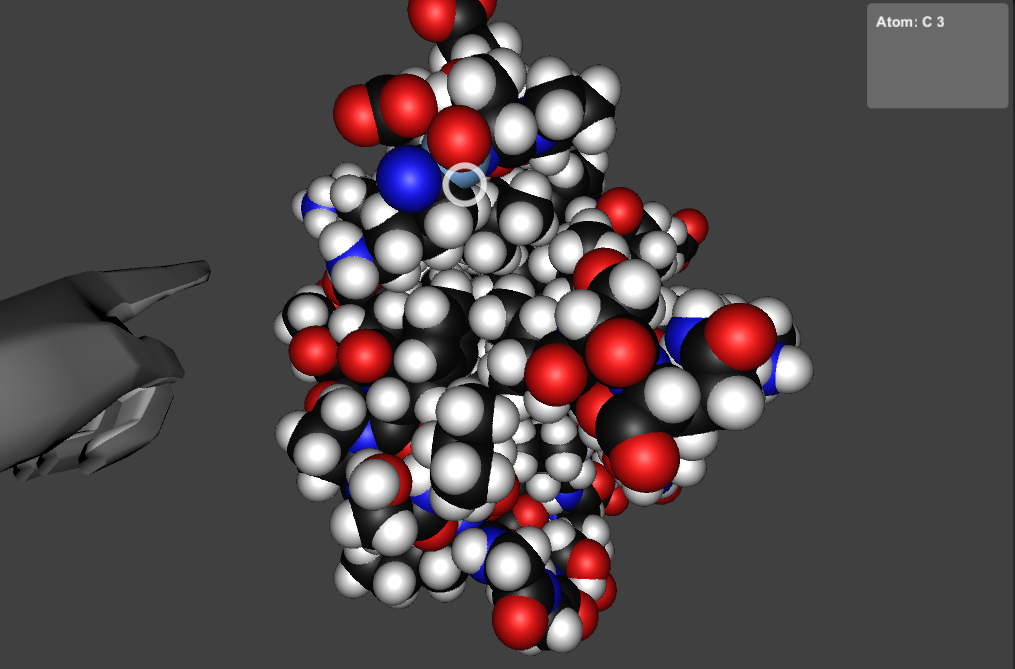
\includegraphics[width=0.8\textwidth]{Figs/pointing.png}
\caption{Pointing with the left hand at the atom. As seen, the cross hair is aimed at the carbon atom number 3, what changed the colour of the sphere from black to bright blue.}
\label{fig:pointing} 
\end{figure}

Since this feature is mostly needed for pointing on an atom, it is available only for Van der Waals and Balls and Sticks representations, as these are the only modes that in fact create objects for each atom. After loading a structure in one of these two styles, user may turn on the Selecting mode by extending left arm forward. In other cases, the left hand does not appear on the screen and the mode is inactive.

Selecting is held by pointing with an index finger at the chosen atom. Pointed sphere changes its color to the bright blue and the atom's name and number is displayed in the right upper corner. That feature enables searching for the requested fragment. If user wants to become familiar with details of the chosen atom, he or she should point at it for few seconds. Targeting is facilitated by a cross hair, which is simultaneously a progress bar indicating the time that left for the atom details presentation (Figure \ref{fig:pointing}). The time buffer protects the user from accidental pointing on other atoms, which could cause chaotic performance.
After successful selection of an atom, its name, element, number, residue and chain is displayed in the upper right corner for 5 seconds (Figure \ref{fig:selecting}). In this time user cannot select another sphere. 

Escaping from the selecting mode is possible by hiding left hand out of \textit{Leap Motion} controller's vision. 

\begin{figure}[!htb]
\centering    
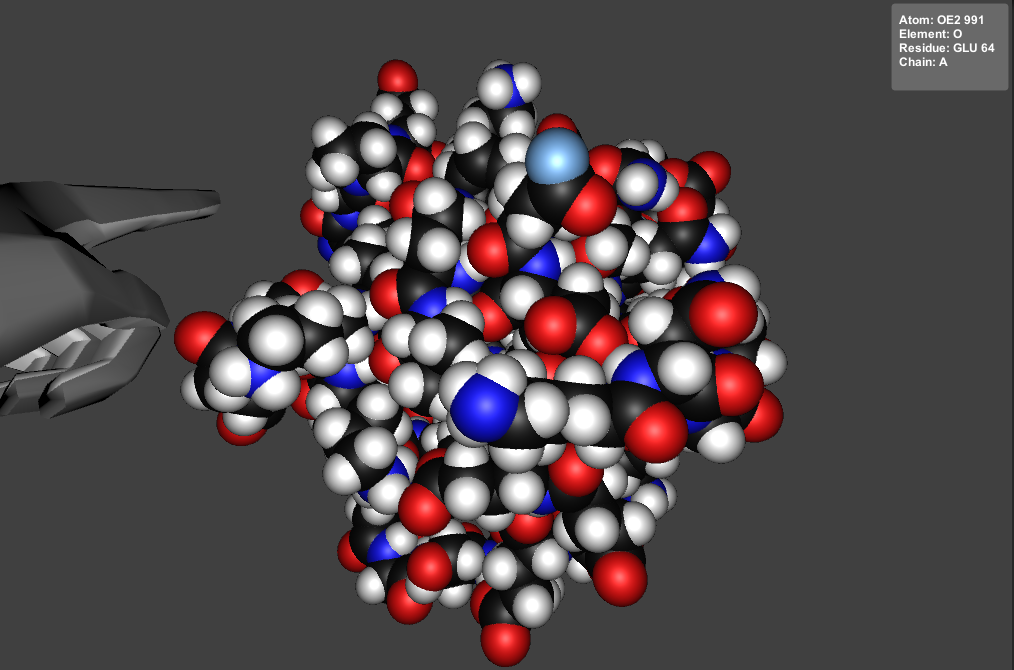
\includegraphics[width=0.8\textwidth]{Figs/selecting.png}
\caption{Selected atom and its details shown in the right upper corner. The cross hair is hidden, as time needed for details presentation has passed and pointing at other atoms is temporarily inactive.}
\label{fig:selecting} 
\end{figure}

\subsection{Exit}

As the re-typing of PDB ID code etc. requires taking off the HMD, there is no way to get back to main menu in single session. Changing of molecule code or chosen setting requires restarting of the program. 

Closing the Molecule VR Viewer may be done by simply clicking the escape key on the keyboard. 


%*******************************************************************************
%*********************************** Fourth Chapter *****************************
%*******************************************************************************

\chapter{Molecule VR Viewer- implementation}\label{chapter4}  %Title of the Fourth Chapter

As previous chapter outlines the result of this work, it does not provide description of methodology needed for creating Molecule VR Viewer. Therefore, this chapter is devoted to programming details, used algorithms and implementation of the project.

%********************************** %First Section  **************************************
\section{\textit{Unity 3D}} %Section - 4.1 

\textit{Unity 3D} game engine provides IDE (Integrated Development Environment) for games and other interactive materials, both in 2D and 3D. In version 5.3, itt enables writing scripts in two languages: UnityScript and C\#. The latter one was used for this work's purpose.

For better understanding of Molecule VR Viewer implementation, the following subsections describe the components needed for creating  materials in \textit{Unity 3D} and explain how do they work.

\subsection{Editor}

Generally saying, \textit{Unity 3D} products are created on two tracks: Editor and Scripting. The first one is editable in main window of application, showing the scenes of the project, their environments and objects.

Objects in \textit{Unity 3D}, called GameObjects, are containers that hold Components and Scripts, which may influence their apperance, properties and actions. For example, every GameObject has the Transform Component, which represents position and orientation i space. The engine serves a huge variety of editable Components, which may be attached to the object, like its physical properties, its material etc. Moreover, some of the general GameObject types containing needed Components are provided by \textit{Unity 3D}, e.g. Cameras, which are responsible for observing the scene, Lights, 3D basic models, UI (User's Interface) elements etc. Additionally, the GameObjects can be stored as templates called Prefabs, from which one can create new instances of the GameObject \cite{Unity16}.

Summing up, Editor mode is the core of the whole project, which enables the developer to combine all of the needed objects, create Scenes, change player settings (like enabling Unity VR Support) and manage it all to create the final product.


\subsection{Scripting}

The second track of developing programs in \textit{Unity 3D} is Scripting. Scripts may be responsible for arranging events and responds in the Gameplay mode, they can influence Components of GameObjects, create and destroy GameObjects etc. As they play huge role in whole mechanism of game or material creating, it is worth knowing their manner of working.

First of all, \textit{Unity} scripts derive from the built-in class MonoBehaviour, which is the base class connecting the script with internal workings of \textit{Unity} engine. By default, the script defines two methods: Start, which is responsible for all initialisations before the gameplay begins, and the next one, Update, which is the place for code that is going to be called once per frame during the gameplay. 

Secondly, it is worth mentioning, that scripts created for \textit{Unity} do not contain constructor functions. This feature is supported by the Editor mode, when script is attached to some GameObject as its Component, which is equal to creating an instance of the class. What is more, variables declared in the class field, which are public, are editable in Editor mode and can be even linked with another GameObject.

Thirdly, scripts are able to access other components that belong to the same GameObject or even to different GameObjects \cite{Unity16}. 

\subsubsection{Event Functions}

Start and Update functions mentioned above are in fact just two examples of the big group of event functions, which are activated  in certain moments of a gameplay. They are the consequence of the fact, that \textit{Unity} does not run the code continuously, script by script. Instead, scripts take control intermittently, when their certain functions are called by \textit{Unity}. After the function's execution, control is passed back to the engine \cite{Unity16}. 

The remaining examples of event functions and their order of execution are shown on the flowchart in Figure \ref{fig:monobehaviour}.

\begin{figure}[p]
\centering    
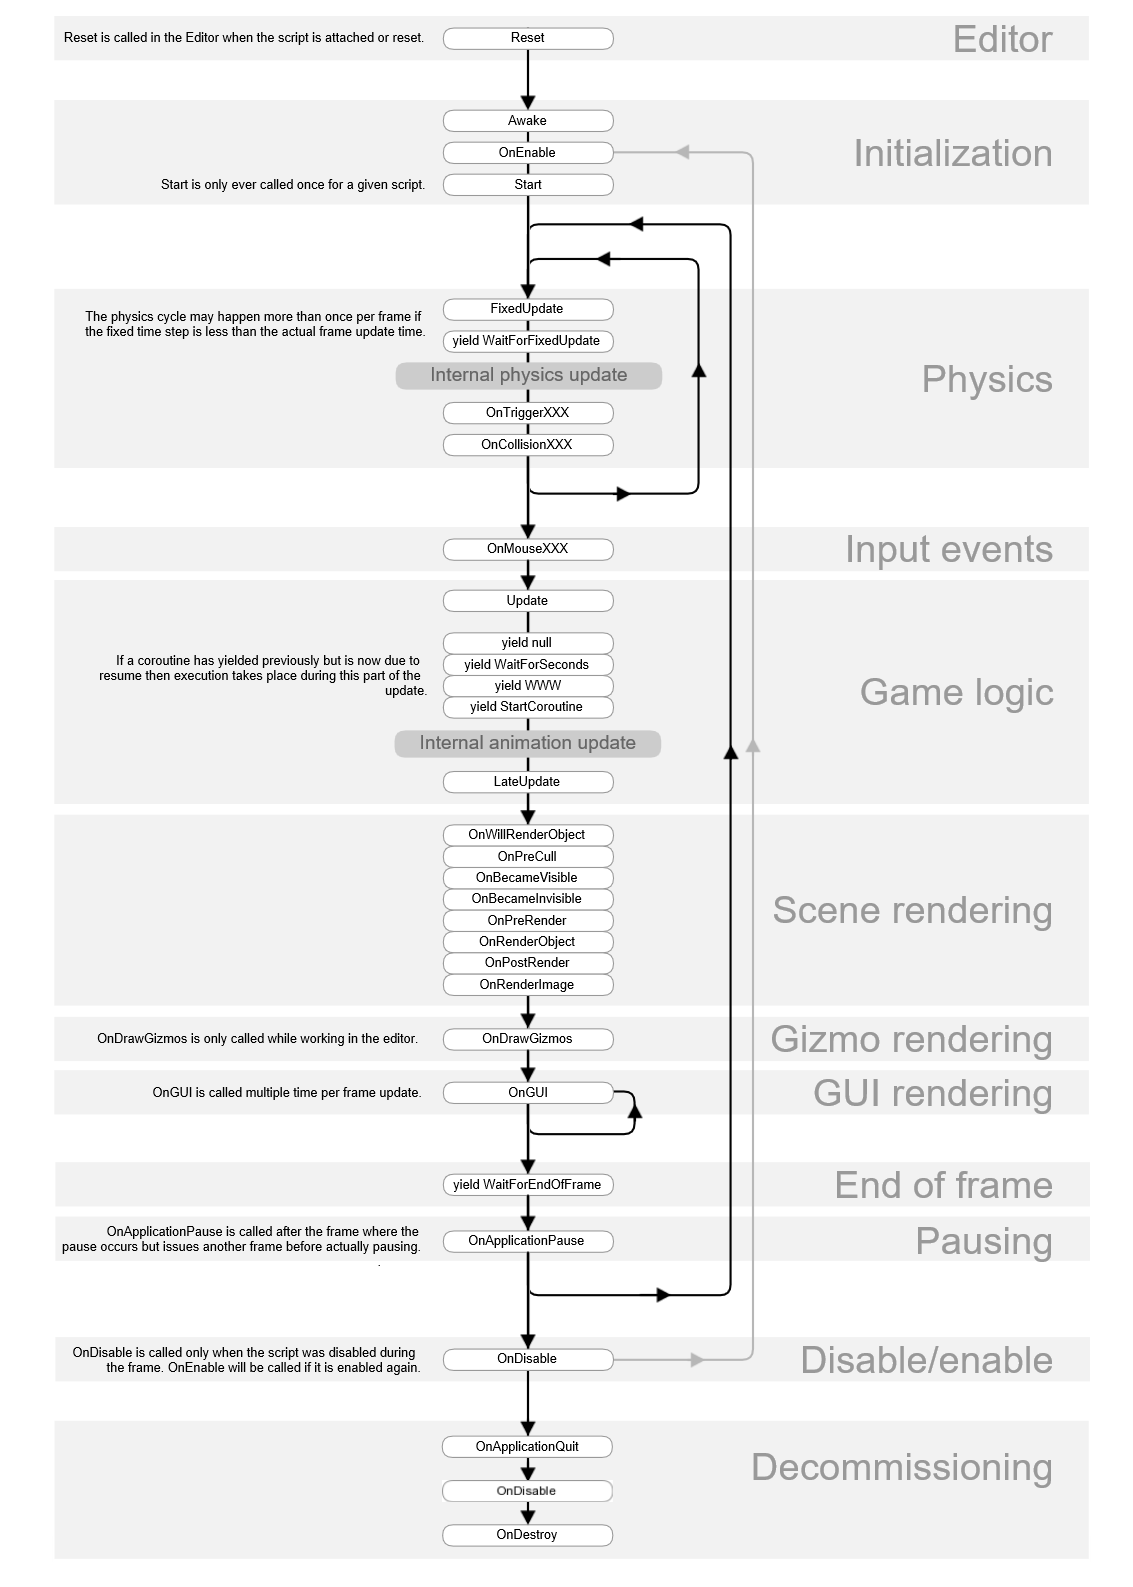
\includegraphics[width=1.0\textwidth]{Figs/monobehaviour_flowchart.png}
\caption{Script lifecycle flowchart with repetitions included \cite{Unity16}.}
\label{fig:monobehaviour} 
\end{figure} 

%********************************** %Second Section  **************************************
\section{\textit{Implementation details}} %Section - 4.2 

Molecule VR Viewer program consists of two scenes- menu and viewer scene- and each one contains the core script that manages all of the functionalities. In this section they are described in details.

\subsection{MainMenu.cs}

MainMenu script is attached to the Main Camera of Menu scene, where the two-dimensional UI (User's Interface) configured in Editor mode, is presented (Figure \ref{fig:mainmenu}). Each UI element has its reference in the script, what enables pulling the data out of it. 

Start function is responsible only for adding the listener to the "Start" button, which is the ButtonFunction method. It it responsible for setting of the feedback message and checking the correctness of entered PDB ID Code, which means its length (PDB codes always have 4 characters) and its actual existence in PDB data base. The latter is done with the HttpWebRequest and HttpWebResponse classes from System.Net library. If the URL address responses, the Viewer scene is loaded with \textit{Unity's} SceneManager. If not, and the WebException occurs, method displays the WebException message on the feedback message presented to the user.

The Update function contains elements responsible for assigning the data inserted by the user and for changing the set of colouring styles depending on which drawing style was chosen. Variables, which are obtained from UI, are held by the Configurator class.

\subsubsection{Configurator.cs}

This class, which does not inherits from MonoBehaviour, initialises four static variables, which are pdbID, hideHydrogens, representationStyle and colouring, with corresponding get and set methods. 

As the user's settings are needed during the entire gameplay, they need to be passed between scenes, which is more challenging than, e.g. communication between objects. The GameObject, where they are set, is no longer needed, therefore using the \textit{Unity's} method DontDestroyOnLoad, which prevents the object from being trashed while loading another scene, is not the best solution. This is why the other way was chosen, which is the usage of static attributes, that are available as long as the application is running. 

\subsection{MoleculeViewer.cs}

Viewer scene, which is loaded after successful request from the PDB server, is managed by the MoleculeViewer script, which constitutes the core of the whole program. It is the only component (except, obviously, Transform component) attached to the GameObject called CameraParent. The reason of that setting is explained later in this section.

In this case, Start function contains all the components needed for creation of structure representation in a way chosen by the user in main menu. First of all, the object of the FileReader class is initialized and its method ReadFile is called.

\subsubsection{FileReader.cs}

This class does not inherit from MonoBehaviour and provides the engine for extracting needed data from PDB database. Therefore, at the very beginning it downloads the PDB file and reads it line by line.

This is a good moment to introduce and describe the PDB file format. Its main property is its linearity- the content is presented in number of lines, with 80 columns per each. First six columns contain a record name, which defines the record type of the line. This is a very useful feature, as every record type is divided into fields, that have standardised positions in the line. Knowing the exact location of interesting data is very convenient in terms of file analysis. Because PDB file may contain a large variety of record types, only those, that were used in this work, are described below \cite{PDB16}.

\begin{itemize}
\item COMPND– macromolecular contents of an entry presented in a form of specification list. Specifications that were used in Molecule VR Viewer are MOLECULE, where the macromolecule name is defined, and CHAIN, which provide list of subunits identifiers, separated by commas.
\item SEQRES– listing of the linearly linked chemical components that form a polymer. For proteins these are amino acids, presented in a form of three-letter codes, and for nucleic acids- their residues. 
\item ATOM- atomic coordinates of an atom that belongs to a standard residue, its name, element symbol, serial number, occupancy, temperature factor, charge and belonging to subunit and residue. XYZ coordinates are in Angstroms. What is important, these records are listed in an ordered way, for proteins from amino to carboxyl terminus, and for nucleic acids- from the 5' to the 3' terminus.
\item HETATM- atomic coordinates of an atom that does not belong to the polymer, its name, element symbol, serial number occupancy, temperature factor, charge and belonging to subunit and residue. Useful especially for prosthetic groups, inhibitors, solvent molecules, metal ions etc.
\item CONECT- specifies connectivity between atoms, mostly for non-standard atoms and disulfide bridges, by assigning to the atom's serial number all the atoms that are bonded with it. 
\item HELIX- specifies the position of helices in a molecule by indication of the initial and ending residue. Helix type is also described by the number corresponding with helix class.
\item SHEET- specifies the position of sheets in a molecule similarly as in HELIX.
\end{itemize}


%\lstset{style=sharpc}
%\begin{lstlisting}
%MonoBehaviour
%\end{lstlisting} 







\nomenclature[z-IDE]{IDE}{Integrated Development Environment}
\nomenclature[z-UI]{UI}{User's Interface}
%\include{Chapter5/chapter5}
%\include{Chapter6/chapter6}
%\include{Chapter7/chapter7}
\begin{thebibliography}{99}
\setlength{\bibsep}{0pt plus 0.3ex}
%\addcontentsline{toc}{chapter}{Bibliografia}
\bibitem{Heim98} Heim M.: \emph{Virtual realism}. Oxford University Press, New York, 1998.

\bibitem{Fuchs92} Fuchs H., Bishop G. et al.: \emph{Research Directions in Virtual Environments}. NFS
Invitational Workshop, Univ. North Carolina, 1992.

\bibitem{Cruz93} Cruz-Neira C.: \emph{Virtual Reality Overview}, SIGGRAPH’93 Course, 23, 1.1-1.18, 1993.

\bibitem{Sherman03} Sherman W., Craig W.: \emph{Understanding Virtual Reality. Interface, Application and Design}. Morgan Kaufmann Publishers, San Francisco, 2003.

\bibitem{Milgram94} Milgram P., Takemura H., Ustumi A., Kishino F: \emph{Augmented Reality: A class of displays on the reality-virtuality continuum}. SPIE proc. Telemanipulator and Telepresence Technologies, 2351: 282-292, 1994.

\bibitem{Olszewski15} Olszewski P.: \emph{Historia wirtualnej rzeczywistości}, 2015. Retrieved January 20, 2016, from [\url{http://www.komputerswiat.pl/centrum-wiedzy-konsumenta/gaming/wszystko-o-wirtualnej-rzeczywistosci/historia-wirtualnej-rzeczywistosci.aspx}].

\bibitem{Mandal13} Mandal S.: \emph{Brief Introduction of Virtual Reality \& its Challenges}. International Journal of Scientific \& Engineering Research, 4, 4: 304-309, 2013.

\bibitem{Lange10} Lange B.S. et al.: \emph{The Potential of Virtual Reality and Gaming to Assist Successful Aging with Disability}. Physical medicine and rehabilitation clinics of North America, 21.2: 339-356, 2010.

\bibitem{Brooks99} Brooks Jr. F.P.: \emph{What’s Real About Virtual Reality?} IEEE Computer Graphics and Applications, 19, 6: 16-27, 1999.

\bibitem{Mazuryk96} Mazuryk T., Gervautz M.: \emph{Virtual Reality History, Applications, Technology and Future}. Institute of Computer Graphics, Vienna University of Technology, 1996. Retrieved January 20, 2016, from [\url{https://www.cg.tuwien.ac.at/research/publications/1996/mazuryk-1996-VRH/TR-186-2-96-06Paper.pdf}].

\bibitem{Wikibook15} Wikibooks contributors: \emph{Cg Programming/Unity/Projection for Virtual Reality}, Wikibooks, The Free Textbook Project, 2015. Retrieved January 25, 2016, from [\url{https://en.wikibooks.org/w/index.php?title=Cg_Programming/Unity/Projection_for_Virtual_Reality&oldid=2988608}].

\bibitem{Oscillada15} Oscillada J.M.: \emph{Comparison Chart of FOV (Field of View) of VR Headsets}, 2015. Retrieved January 20, 2016, from [\url{http://www.virtualrealitytimes.com/2015/05/24/chart-fov-field-of-view-vr-headsets/}].

\bibitem{Lacrama07} Lacrama, Dan L.; Fera D.: \emph{Virtual Reality}. Ann. Univ. Tibiscus, Computer Science Series V, 1: 137-144, 2007.

\bibitem{Parisi15} Parisi T.: \emph{Learning Virtual Reality}. O'Reily Media, Sebastopol, 2015.

\bibitem{Gobbetti99} Gobbetti E., Scateni R.: \emph{Virtual reality: Past, present, and future}. Virtual Environments in Clinical Psychology and Neuroscience: Methods and Techniques in Advanced Patient-Therapist Interaction, 3-20, IOS, Amsterdam, 2015.

\bibitem{Oculus16} \emph{Oculus Rift Documentation}, 2016. Retrieved January 27, 2016, from [\url{https://developer.oculus.com/documentation/}].

\bibitem{Feelreal16} \emph{FeelReal official website}, 2016. Retrieved January 27, 2016, from [\url{http://feelreal.com/smells}].

\bibitem{Marco15} Marco J.: \emph{List of Haptic Controllers under Development for Virtual Reality}, 2015. Retrieved January 27, 2016, from [\url{http://www.virtualrealitytimes.com/2015/03/13/list-of-haptic-controllers-virtual-reality/}].

\bibitem{Roadtovr14} \emph{Overview of Positional Tracking Technologies for Virtual Reality}, 2014. Retrieved February 06, 2016, from [\url{http://www.roadtovr.com/overview-of-positional-tracking-technologies-virtual-reality/}].

\bibitem{Weichert13} Weichert F., Bachamn D., Rudak B., Fisseler D.: \emph{Analysis of the Accuracy and Robustness of the Leap Motion Controller}. Sensors (Basel, Switzerland), 13(5): 6380-6393, 2013.

\bibitem{Leap16} \emph{Leap Motion Documentation}, 2016. Retrieved May 06, 2016, from [\url{https://developer.leapmotion.com/documentation/}].

\bibitem{Singal15} Singal N.: \emph{Magic Realism}, 2014. Business Today, November 8, 205-208, 2015.

\bibitem{Goodsell04} Goodsell D.S.: \emph{Bionanotechnology : lessons from nature}. Wiley-Liss, Inc., Hoboken, New Jersey, 2004. 

\bibitem{Gruca10} Gruca A.: \emph{Bioinformatyczne bazy danych}. Wydawnictwo PJWSTK, Warszawa 2010. 

\bibitem{Anderson99} Anderson A., Weng Z.: \emph{VRDD: Applying virtual reality visualization to protein docking and design}. Journal of Molecular Graphics and Modelling, 17: 180-186, 1999.

\bibitem{Schulze11} Schulze J.P. et al.: \emph{Advanced applications of virtual reality}. Advances in Computers, 82: 217-260. Academic Press, Burlington 2011.

\bibitem{Herisson05} Hérisson J. et al.: \emph{3D visualization and virtual exploration of genomic sequences}. Data Science Journal, 4: 82-91, 2005.

\bibitem{Hamdi08} Hamdi M. et al.: \emph{Prototyping bio-nanorobots using molecular dynamics simulation and virtual reality}. Microelectronics Journal, 39: 190–201, 2008.

\bibitem{Norrby15} Norrby M. et al.: \emph{Molecular Rift: Virtual Reality for Drug Designers}. Journal of Chemical Information and Modeling, 55: 2475-2484, 2015.

\bibitem{Koltun65} Koltun W.L.: \emph{Space filling atomic units and connectors for molecular models}. U. S. Patent 3170246, 1965.

\bibitem{Rasmol16} \emph{Rasmol v2.6 Manual}, 2016. Retrieved May 06, 2016, from [\url{http://life.nthu.edu.tw/~fmhsu/rasframe/TOC.HTM}].


\end{thebibliography}



% ********************************** Back Matter *******************************
% Backmatter should be commented out, if you are using appendices after References
%\backmatter

% ********************************** Bibliography ******************************
%\begin{spacing}{0.9}

% To use the conventional natbib style referencing
% Bibliography style previews: http://nodonn.tipido.net/bibstyle.php
% Reference styles: http://sites.stat.psu.edu/~surajit/present/bib.htm

%\bibliographystyle{apalike}
%\bibliographystyle{unsrt} % Use for unsorted references  
%\bibliographystyle{plainnat} % use this to have URLs listed in References
%\cleardoublepage
%\bibliography{References/references} % Path to your References.bib file


% If you would like to use BibLaTeX for your references, pass `custombib' as
% an option in the document class. The location of 'reference.bib' should be
% specified in the preamble.tex file in the custombib section.
% Comment out the lines related to natbib above and uncomment the following line.

%\printbibliography[heading=bibintoc, title={References}]


%\end{spacing}

% ********************************** Appendices ********************************

%\begin{appendices} % Using appendices environment for more functunality

%% ******************************* Thesis Appendix A ****************************
\chapter{How to install \LaTeX} 

\section*{Windows OS}

\subsection*{TeXLive package - full version}
\begin{enumerate}
\item	Download the TeXLive ISO (2.2GB) from\\
\href{https://www.tug.org/texlive/}{https://www.tug.org/texlive/}
\item	Download WinCDEmu (if you don't have a virtual drive) from \\
\href{http://wincdemu.sysprogs.org/download/}
{http://wincdemu.sysprogs.org/download/}
\item	To install Windows CD Emulator follow the instructions at\\
\href{http://wincdemu.sysprogs.org/tutorials/install/}
{http://wincdemu.sysprogs.org/tutorials/install/}
\item	Right click the iso and mount it using the WinCDEmu as shown in \\
\href{http://wincdemu.sysprogs.org/tutorials/mount/}{
http://wincdemu.sysprogs.org/tutorials/mount/}
\item	Open your virtual drive and run setup.pl
\end{enumerate}

or

\subsection*{Basic MikTeX - \TeX~ distribution}
\begin{enumerate}
\item	Download Basic-MiK\TeX (32bit or 64bit) from\\
\href{http://miktex.org/download}{http://miktex.org/download}
\item	Run the installer 
\item	To add a new package go to Start >> All Programs >> MikTex >> Maintenance (Admin) and choose Package Manager
\item	Select or search for packages to install
\end{enumerate}

\subsection*{TexStudio - \TeX~ editor}
\begin{enumerate}
\item	Download TexStudio from\\
\href{http://texstudio.sourceforge.net/\#downloads}
{http://texstudio.sourceforge.net/\#downloads} 
\item	Run the installer
\end{enumerate}

\section*{Mac OS X}
\subsection*{MacTeX - \TeX~ distribution}
\begin{enumerate}
\item	Download the file from\\
\href{https://www.tug.org/mactex/}{https://www.tug.org/mactex/}
\item	Extract and double click to run the installer. It does the entire configuration, sit back and relax.
\end{enumerate}

\subsection*{TexStudio - \TeX~ editor}
\begin{enumerate}
\item	Download TexStudio from\\
\href{http://texstudio.sourceforge.net/\#downloads}
{http://texstudio.sourceforge.net/\#downloads} 
\item	Extract and Start
\end{enumerate}


\section*{Unix/Linux}
\subsection*{TeXLive - \TeX~ distribution}
\subsubsection*{Getting the distribution:}
\begin{enumerate}
\item	TexLive can be downloaded from\\
\href{http://www.tug.org/texlive/acquire-netinstall.html}
{http://www.tug.org/texlive/acquire-netinstall.html}.
\item	TexLive is provided by most operating system you can use (rpm,apt-get or yum) to get TexLive distributions
\end{enumerate}

\subsubsection*{Installation}
\begin{enumerate}
\item	Mount the ISO file in the mnt directory
\begin{verbatim}
mount -t iso9660 -o ro,loop,noauto /your/texlive####.iso /mnt
\end{verbatim}

\item	Install wget on your OS (use rpm, apt-get or yum install)
\item	Run the installer script install-tl.
\begin{verbatim}
	cd /your/download/directory
	./install-tl
\end{verbatim}
\item	Enter command `i' for installation

\item	Post-Installation configuration:\\
\href{http://www.tug.org/texlive/doc/texlive-en/texlive-en.html\#x1-320003.4.1}
{http://www.tug.org/texlive/doc/texlive-en/texlive-en.html\#x1-320003.4.1} 
\item	Set the path for the directory of TexLive binaries in your .bashrc file
\end{enumerate}

\subsubsection*{For 32bit OS}
For Bourne-compatible shells such as bash, and using Intel x86 GNU/Linux and a default directory setup as an example, the file to edit might be \begin{verbatim}
edit $~/.bashrc file and add following lines
PATH=/usr/local/texlive/2011/bin/i386-linux:$PATH; 
export PATH 
MANPATH=/usr/local/texlive/2011/texmf/doc/man:$MANPATH;
export MANPATH 
INFOPATH=/usr/local/texlive/2011/texmf/doc/info:$INFOPATH;
export INFOPATH
\end{verbatim}
\subsubsection*{For 64bit OS}
\begin{verbatim}
edit $~/.bashrc file and add following lines
PATH=/usr/local/texlive/2011/bin/x86_64-linux:$PATH;
export PATH 
MANPATH=/usr/local/texlive/2011/texmf/doc/man:$MANPATH;
export MANPATH 
INFOPATH=/usr/local/texlive/2011/texmf/doc/info:$INFOPATH;
export INFOPATH

\end{verbatim}



%\subsection{Installing directly using Linux packages} 
\subsubsection*{Fedora/RedHat/CentOS:}
\begin{verbatim} 
sudo yum install texlive 
sudo yum install psutils 
\end{verbatim}


\subsubsection*{SUSE:}
\begin{verbatim}
sudo zypper install texlive
\end{verbatim}


\subsubsection*{Debian/Ubuntu:}
\begin{verbatim} 
sudo apt-get install texlive texlive-latex-extra 
sudo apt-get install psutils
\end{verbatim}

%% ******************************* Thesis Appendix B ********************************

\chapter{Installing the CUED class file}

\LaTeX.cls files can be accessed system-wide when they are placed in the
<texmf>/tex/latex directory, where <texmf> is the root directory of the user’s \TeX installation. On systems that have a local texmf tree (<texmflocal>), which
may be named ``texmf-local'' or ``localtexmf'', it may be advisable to install packages in <texmflocal>, rather than <texmf> as the contents of the former, unlike that of the latter, are preserved after the \LaTeX system is reinstalled and/or upgraded.

It is recommended that the user create a subdirectory <texmf>/tex/latex/CUED for all CUED related \LaTeX class and package files. On some \LaTeX systems, the directory look-up tables will need to be refreshed after making additions or deletions to the system files. For \TeX Live systems this is accomplished via executing ``texhash'' as root. MIK\TeX users can run ``initexmf -u'' to accomplish the same thing.

Users not willing or able to install the files system-wide can install them in their personal directories, but will then have to provide the path (full or relative) in addition to the filename when referring to them in \LaTeX.



%\end{appendices}

% *************************************** Index ********************************
%\printthesisindex % If index is present

\end{document}
